\documentclass[usenames,dvipsnames,notheorems]{beamer}

\usefonttheme[onlymath]{serif}

% silence annoying warnings
\usepackage{silence}
\usepackage{caption}
\WarningFilter{remreset}{The remreset package}
\usepackage{xcolor}
\usepackage{algorithm}
\usepackage{algorithmic}
\usepackage{centernot}
\usepackage{dsfont}

\input{macros/math}
\input{macros/plots}

\usepackage{simplebeam}
\usetheme{simplebeamer}

\usetikzlibrary{shapes, arrows}
\usetikzlibrary{decorations.pathreplacing, calligraphy}

% node styles
\tikzstyle{Input}=[minimum size=0.5cm, fill=none, line width = 0.5mm, draw=black, shape=circle, text=black]
\tikzstyle{Hidden}=[minimum size=0.4cm, fill=blue, line width = 0.5mm, draw=blue, shape=circle, text=black]
\tikzstyle{Splits}=[inner sep=0.03cm, minimum size=0.3cm, line width = 0.3mm, draw=blue, shape=circle, text=black]
\tikzstyle{Output}=[minimum size=0.3cm, fill=white, line width = 0.5mm, draw=black, shape=circle, text=black]

% Edge styles
\tikzstyle{arrow}=[line width = 0.5mm]

% bib resources

\addbibresource[]{refs.bib}

\title{Convex Analysis of Non-Convex Neural Networks}
\author{Aaron Mishkin\\ \vspace{1.5ex} {\small Supervised by Mert Pilanci}}
\collaborators{
	\includegraphics[width=0.3\linewidth]{assets/aaron_excited.jpeg}
	\includegraphics[width=0.3\linewidth]{assets/mert.jpg}
}

\titlegraphic{\includegraphics[width=0.4\textwidth]{assets/SUSig_2color_Stree_Left.eps}}

\newcommand{\horizontalrule}{
	{
			\vspace{-0.5em}
			\center \rule{\textwidth}{0.1em}
			\vspace{-0.2em}
		}
}

\newcommand{\red}[1]{\textcolor{Red}{#1}}
\newcommand{\green}[1]{\textcolor{ForestGreen}{#1}}
\newcommand{\blue}[1]{\textcolor{DarkBlue}{#1}}
\newcommand{\purple}[1]{\textcolor{Magenta}{#1}}

\definecolor{bad}{HTML}{eb6223}
\definecolor{good}{HTML}{9434ed}

\newcommand{\bad}[1]{\textcolor{bad}{#1}}
\newcommand{\good}[1]{\textcolor{good}{#1}}

\definecolor{sanddune}{rgb}{0.59, 0.44, 0.09}
\definecolor{byzantine}{rgb}{0.59, 0.44, 0.09}
\definecolor{ultramarine}{rgb}{0.07, 0.04, 0.56}
\definecolor{brightpink}{rgb}{1.0, 0.0, 0.5}

% toggle plotting tikz
\def\showtikz{}

%\logo{\includegraphics[height=0.5cm]{assets/Block_S_2_color.eps}}

%\institute{Stanford University}
\frenchspacing
\date{}

\begin{document}

\maketitle
%% main content starts %%

\setbeamercolor{background canvas}{bg=LightCyan}

\begin{frame}{}
    \begin{center}
        \huge 1. Motivation: Convexity and Deep Learning
    \end{center}
\end{frame}
\setbeamercolor{background canvas}{bg=white}

\begin{frame}{Motivation: Thirteen Years Since AlexNet}

    {
        \large \textbf{13 Years Ago}: AlexNet won ILSVRC 2012 and started
        the modern ``deep learning'' era of machine learning.
    }
    \pause

    \vspace{0.5em}

    \horizontalrule

    \vspace{0.5em}

    AlexNet improved over the next best model by \( \approx 10\% \) (top-5).

    \vspace{1em}
    \pause

    \textbf{Key Techniques}:
    \pause
    \begin{itemize}
        \item ``a \good{large}, deep convolutional neural network''
              \pause
        \item ``a very \good{efficient} GPU implementation of convolutional
              nets''
              \pause
        \item ``'dropout', a recently-developed \good{regularization} method
              that proved to be very effective''
    \end{itemize}
    \pause
    \vspace{1ex}
    \begin{center}
        \large
        \good{Not so different from today\ldots}
    \end{center}

    \source{https://image-net.org/challenges/LSVRC/2012/results.html\#abstract}
\end{frame}

\begin{frame}{Motivation: ImageNet Today}

    \begin{center}
        \large AlexNet won with \( \bad{84.69\%} \) top-five accuracy \citep{krizhevsky2012alexnet}.
    \end{center}

    \pause
    \horizontalrule

    \begin{center}
        \large Today, models get \( \good{99.02\%} \) top-5 accuracy \citep{yuan2021florence}!

        \vspace{3em}

        (Using all sorts of tricks like pre-training, transformers, etc.)
    \end{center}
\end{frame}

\begin{frame}{Motivation: DALL$\cdot$E 2}
    \begin{center}
        We've developed amazing deep learning tools since AlexNet.
    \end{center}
    \pause
    \vspace{1ex}

    \begin{figure}[]
        \centering
        \includegraphics[width=0.6\linewidth]{assets/bowl_of_soup.jpg}
        \caption*{Generated by DALL$\cdot$E 2}%
    \end{figure}

    \begin{center}
        \textit{A bowl of soup that is a portal to another
            dimension as digital art.}
    \end{center}

    \source{https://openai.com/dall-e-2/}

\end{frame}

\begin{frame}{Motivation: Cost of Training DALL$\cdot$E 2}

    \begin{center}
        \large
        DALL$\cdot$E 2 has 5.5 billion parameters and took \red{billions} of Adam
        iterations to fit \citep{ramesh2022dalle}.
    \end{center}

    \pause
    \horizontalrule

    \begin{center}
        \large
        But this is small compared to recent LLMs!
    \end{center}

    \pause
    \vspace{2ex}

    Consider OpenAI's \good{GPT-4 model}:
    \vspace{1ex}
    \pause

    \begin{itemize}
        \item GPT-4 has \bad{\( 1.8 \) trillion} parameters;
              \vspace{0.5ex}
              \pause

        \item It was trained on \bad{\( \approx 13 \) trillion} tokens;
              \vspace{0.5ex}
              \pause

        \item Training used \bad{25,000 A100s} for 90 to 100 days;
              \vspace{0.5ex}
              \pause

        \item At \$1 per A100 hour, GPT-4 cost \bad{\( \approx \$63 \) million} dollars.
    \end{itemize}

    \source{https://the-decoder.com/gpt-4-architecture-datasets-costs-and-more-leaked/}

\end{frame}

\begin{frame}{Motivation: Challenges of Non-Convexity}

    \textbf{Takeaway}:
    Modern deep learning models are \bad{huge} and \bad{extremely expensive}
    to train, but they have \good{tremendous impact}.
    \pause
    \vspace{1.0ex}

    \hspace{1em} \( \hookrightarrow \) ChatGPT is
    the fastest-adopted piece of software in history!

    \pause
    \horizontalrule
    \vspace{-1ex}

    \begin{figure}[]
        \centering
        \ifdefined\showtikz
            \input{assets/non_convex.tex}
        \else
            \Huge Non-Convex Figure
        \fi
    \end{figure}

    \vspace{-1ex}
    \textbf{Challenges of Non-Convexity}:
    \vspace{0.25ex}
    \pause

    \begin{itemize}
        \item \bad{Optimization}: saddle-points, local minima,
              slow convergence.

              \vspace{0.5em}
              \pause

        \item \bad{Optimality Conditions}: stationarity
              \( \centernot \implies \) optimality.

              \vspace{0.5em}
              \pause

        \item \bad{Mathematical Tools}: No subgradients, no separating
              hyperplanes, (usually) non-zero duality gap.
    \end{itemize}

    \source{www.theguardian.com/technology/2023/feb/02/chatgpt-100-million-users-open-ai-fastest-growing-app}

\end{frame}

\begin{frame}{Motivation: Convexity and Deep Learning}

    \textbf{Key Question}: How can we overcome \bad{non-convexity} to get
    \underline{better optimization} and \underline{fundamental theory} for neural networks?

    \pause
    \vspace{2ex}

    \textbf{This Thesis}: By creating and studying \good{convex reformulations}.

    \pause
    \vspace{2ex}

    %! TEX root = ../../main.tex

%% illustration of relations between hypothesis classes. 

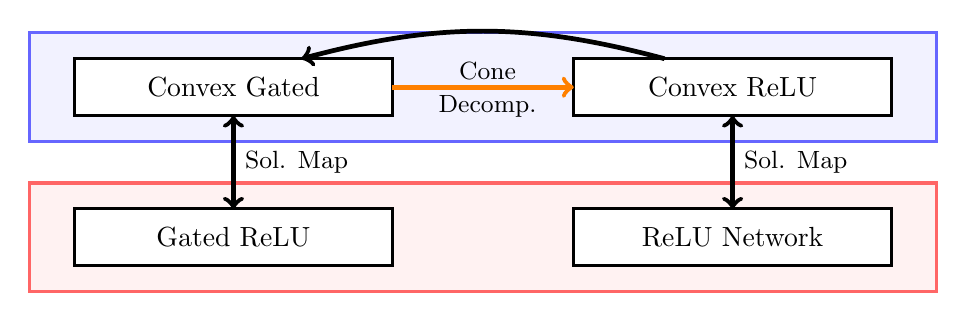
\begin{tikzpicture}[scale=1,
    ]
    \begin{axis}[width=1.1\linewidth, height=5cm,
            axis lines=none,  % don't print axis lines
            yticklabels={,,}, xticklabels={,,},
            ymin=-0.2, ymax=10.2, x axis line style={-},
            xmin=-0.2, xmax=20.2, y axis line style={-},
        ]

        \filldraw[color=blue!60, fill=blue!5, line width=0.4mm](axis cs:0,5.8) rectangle (axis cs:20, 10);
        \filldraw[color=red!60, fill=red!5, line width=0.4mm](axis cs:0,0) rectangle (axis cs:20, 4.2);

        % non-convex models
        \filldraw[line width=0.4mm, fill=white](axis cs:1,1) rectangle (axis cs:8, 3.2) node[pos=.5] {Gated ReLU};
        \filldraw[line width=0.4mm, fill=white](axis cs:12,1) rectangle (axis cs:19, 3.2) node[pos=.5] {ReLU Network};

        % convex models
        \filldraw[line width=0.4mm, fill=white](axis cs:1,6.8) rectangle (axis cs:8, 9) node[pos=.5] {Convex Gated};
        \filldraw[line width=0.4mm, fill=white](axis cs:12,6.8) rectangle (axis cs:19, 9) node[pos=.5] {Convex ReLU};

        \draw [<->, solid, draw=black, line width = 0.6mm] (axis cs:4.5,3.2) -- (axis cs:4.5,6.8) node[right, pos=0.5] {\small Sol. Map};

        \draw [<->, solid, draw=black, line width = 0.6mm] (axis cs:15.5,3.2) -- (axis cs:15.5,6.8)  node[right, pos=0.5] {\small Sol. Map};

        \draw [<-, solid, draw=black, line width = 0.6mm] (axis cs:6,9) to [bend left=15] (axis cs:14, 9);

        \draw [->, solid, draw=orange, line width = 0.6mm] (axis cs:8,7.9) -- (axis cs:12,7.9);
        \node[align=center] at (axis cs:10.1, 7.8) {\small Cone\\ \small Decomp.};
    \end{axis}

\end{tikzpicture}%


    \pause
    \vspace{1.5ex}

    \hspace{1em} \( \hookrightarrow \) This approach yields
    new \good{algorithms} and new \good{insights}!
\end{frame}

%\begin{frame}{Overview: Challenges of Non-Convexity}
%    \begin{center}
%        \Large
%        Non-convexity makes extensions to MLPs \bad{hard}!
%    \end{center}

%    %\begin{itemize}
%    %    \item \textbf{Certificates}: stationary points are global minima.

%    %          \pause
%    %    \item \textbf{Model Churn}: strict/strong convexity gives uniqueness.

%    %          \pause
%    %    \item \textbf{Tuning}: line-search, full-batch methods, acceleration, etc.
%    %\end{itemize}

%\end{frame}

\begin{frame}{Motivation: Two Layer Models}

    \begin{center}
        \large
        We primarily study \bad{two-layer} ReLU networks.
    \end{center}

    \pause
    \horizontalrule
    %\vspace{1ex}

    Two-layer ReLU models are \textbf{foundational building blocks}:
    \pause
    \vspace{1ex}
    \begin{itemize}
        \item They are the basic units of models like \good{MLPs} and \good{CNNs}\ldots
              \pause
              \vspace{0.5ex}

        \item \ldots and \good{layer-wise training} is fast and generalizes well
              \citep{belilovsky2019layer}.

              \pause
              \vspace{0.5ex}

        \item Two-layer networks can model \good{self-attention}
              \citep{sahiner2022attention}\ldots

              \pause
              \vspace{0.5ex}

        \item \ldots and are basic components of standard \good{transformer
                  blocks}.

              \pause
              \vspace{0.5ex}

        \item They were key to word-embeddings (\good{Word2Vec})
              \citep{mikolov2023word}\ldots
              \pause
              \vspace{0.5ex}

        \item \ldots and are widely used in \good{reinforcement learning}
              \citep{gaur2023global} and for prediction on \good{edge devices}
              \citep{teerapittayanon2017distributed}.

    \end{itemize}
    \pause
    \vspace{1ex}

    \begin{center}
        \large
        \textbf{More Importantly}: What can we achieve with two-layers?
    \end{center}

\end{frame}

\begin{frame}{Motivation: Tuning-Free Training Algorithms}

    Training neural networks involves many \bad{hyper-parameters}.
    \pause
    \vspace{0.5ex}
    \begin{itemize}
        \item \textbf{Step-Size}: too small \( \implies \) very slow convergence.
              \pause
              \vspace{0.5ex}
        \item \textbf{Step-Size}: too big \( \implies \) catastrophic failure.
              \pause
              \vspace{0.5ex}
        \item Not to mention batch-size, momentum, decay schedules, \ldots
    \end{itemize}
    \pause

    \begin{figure}
        \centering
        \includegraphics[width=0.8\textwidth]{assets/synthetic_classification.png}
    \end{figure}
    \pause

    Convex reformulations enable \good{parameter-free} global optimization!

\end{frame}

\begin{frame}{Motivation: Theory of Neural Networks}

    {\large \underline{Going Beyond Optimization}}
    \vspace{1.5ex}

    \begin{itemize}
        \item Better optimization is important for \textbf{practitioners}.
              \pause
              \vspace{1ex}

              \begin{itemize}
                  \item Less \bad{babysitting} means \good{faster, cheaper, better} training.
              \end{itemize}
              \pause
              \vspace{1.5ex}

        \item But expensive hyper-parameter tuning hasn't prevented neural
              networks from being deployed \textbf{everywhere}.
              \pause
              \vspace{1ex}

              \begin{itemize}
                  \item They're in our \good{cars} (self-driving), \good{phones} (Face ID),
                        \bad{classrooms} (ChatGPT), and even our \good{research} (ChatGPT again)!
              \end{itemize}
              \pause
              \vspace{1.5ex}

        \item Understanding neural networks is important for \textbf{everyone}.
              \pause
              \vspace{1ex}

              \begin{itemize}
                  \item Neural network theory is necessary for
                        \good{safety}, \good{reliability}, and \good{future
                            advances}.
              \end{itemize}
    \end{itemize}

    \hspace{1ex}
    \pause

    {\large Let's look at some examples\ldots}

\end{frame}

\begin{frame}{Motivation: Global Optima and Generalization}

    \begin{itemize}
        \item Suppose we could take 10,000 models from the set of
              \good{globally optimal} neural networks given a fixed training set.
              \pause
        \item \textbf{Q}: Are they going to generalize differently?
    \end{itemize}
    \pause

    \begin{figure}[t]
        \centering
        \includegraphics[width=0.48\linewidth]{assets/dist_paper_monks-1.pdf}
        \includegraphics[width=0.48\linewidth]{assets/dist_paper_planning.pdf}
    \end{figure}

    \pause

    \textbf{Conclusion}: We need to distinguish between global optima!

\end{frame}

\begin{frame}{Motivation: Structure of Solution Sets}

    \textbf{Q}: What is the structure of the optimal set?
    \pause
    \begin{itemize}
        \item Are the solutions \bad{discrete} or \good{highly connected}?
              \pause
        \item Are connected components \bad{disorganized} or very \good{structured}?
              \pause
    \end{itemize}
    
    \begin{columns}
        \column{0.4\textwidth} 
        \includegraphics[width=1\linewidth]{assets/convex_polytope.png}

        \textbf{A}: It's a convex polytope!

        \pause

        \column{0.65\textwidth}%
        \includegraphics[width=1.1\linewidth]{assets/solution_sets_vis_270.png}
        
        \vspace{1.5ex}
        \textbf{Non-Convex} solution set maps the polytope to a manifold.

    \end{columns}
    
    \vspace{2ex}
    \pause

    \hspace{1em} \( \hookrightarrow \) A \good{connectivity hierarchy}
    emerges with network width!
\end{frame}

%\begin{frame}{Motivation: Dispelling Myths}

%    \begin{center}
%        \large What can we do beyond better optimization algorithms?
%    \end{center}

%    \vspace{-2.5ex}
%    \pause
%    \horizontalrule
%    \vspace{-1ex}

%    We disprove \textbf{long-standing myths} in neural network theory!

%    \pause
%    \vspace{1ex}

%    \begin{itemize}
%        \item ``Optimal neural networks are unique up to model symmetries,
%              like permutations or neuron splitting''.
%              \pause
%              \vspace{0.5ex}
%              \begin{itemize}
%                  \item \bad{False!} But the optimal \good{neuron directions} are unique!
%              \end{itemize}
%              \pause
%              \vspace{0.75ex}

%        \item ``All optimal networks generalize the same''.
%              \pause
%              \vspace{0.5ex}
%              \begin{itemize}
%                  \item \bad{False!} The optimal set admits a \good{clear
%                            characterization} and distinct members of this set can
%                        generalize \good{very differently}.
%              \end{itemize}
%              \pause
%              \vspace{0.75ex}

%        \item ``All the globally optimal neural networks are connected''.
%              \pause
%              \vspace{0.5ex}
%              \begin{itemize}
%                  \item \bad{False!} But a \good{connectivity hierarchy}
%                        emerges as the network width increases.
%              \end{itemize}
%              \pause
%    \end{itemize}

%    \vspace{0.75ex}

%    We prove this and more by exactly characterizing the \textbf{optimal set}.

%\end{frame}

%\begin{frame}{Motivation: Compression and Neuron Pruning}

%    \textbf{Question}: What does the optimal set tell us about \bad{model
%        compression} and \bad{neuron pruning}?

%    \pause
%    \vspace{1ex}

%    \textbf{Answer}: Tight bounds on \good{model width} and an \good{optimal
%        neuron pruning} algorithm in poly-time.

%    \pause

%    \begin{figure}
%        \centering
%        \includegraphics[width=0.9\textwidth]{assets/mnist_pruning_acc.pdf}
%    \end{figure}

%\end{frame}

%\begin{frame}{Overview: Power of Convexity}

%    \begin{figure}
%        \centering
%        \includegraphics[width=0.9\textwidth]{assets/lars.pdf}
%    \end{figure}
%    \vspace{-0.5ex}

%    \textbf{Consider the Lasso:}
%    \pause
%    \vspace{0.5ex}
%    \begin{enumerate}
%        \item \textbf{Optimal Sets}: we have an exact \good{polyhedral
%                  characterization} and simple criteria for \good{uniqueness}
%              (general position) \citep{tibshirani2013unique}.
%              \pause
%              \vspace{0.5ex}

%        \item \textbf{Regularization Paths}: we know the (min-norm) solution
%              path is \good{continuous} and \good{piece-wise linear}
%              \citep{osborne2000new}.
%              \pause
%              \vspace{0.5ex}

%        \item \textbf{Algorithms}: we have efficient algorithms for
%              \good{homotopy} \citep{efron2004least} and computing \good{minimal
%                  solutions} \citep{tibshirani2013unique}.
%    \end{enumerate}

%\end{frame}{}

%\begin{frame}{Overview: Challenges of Non-Convexity}
%    \begin{center}
%        \Large
%        Non-convexity makes extensions to MLPs \bad{hard}!
%    \end{center}

%    \begin{figure}[]
%        \centering
%        \ifdefined\showtikz
%            \input{assets/non_convex.tex}
%        \else
%            \Huge Non-Convex Figure
%        \fi
%    \end{figure}

%    \pause
%    \begin{itemize}

%        \item \textbf{Optimization}: gradient methods escape saddle-points
%              \bad{slowly} and may converge to \bad{sub-optimal} local minima.
%              \vspace{1em}
%              \pause

%        \item \textbf{Optimality Conditions}: Stationarity
%              \( \centernot \implies \) optimality.
%              We have no global \bad{optimality criteria} and no \bad{certificates}.

%              \vspace{1em}
%              \pause

%        \item \textbf{Mathematical Tools}: We lose most of convex analysis
%              and have to work with \bad{Clarke stationary points}, etc.
%    \end{itemize}

%    %\begin{itemize}
%    %    \item \textbf{Certificates}: stationary points are global minima.

%    %          \pause
%    %    \item \textbf{Model Churn}: strict/strong convexity gives uniqueness.

%    %          \pause
%    %    \item \textbf{Tuning}: line-search, full-batch methods, acceleration, etc.
%    %\end{itemize}

%\end{frame}

\begin{frame}{Overview: Big Idea}

    {
        \large
        \bad{Overall Problem}: neural networks are hard to train and even
        harder to analyze because of non-convexity.
    }

    \pause
    \vspace{0.5em}
    \horizontalrule
    \vspace{0.5em}

    {
        \large \good{Thesis Goal}: leverage \textbf{convex reformulations}
        of neural networks to break the barrier of non-convexity and obtain,
        \vspace{1ex}
        \pause

        \begin{itemize}
            \item faster, more reliable optimization algorithms for training
                  shallow neural networks;
                  \pause
                  \vspace{1ex}

            \item a variational theory for the optimal set, solution path,
                  and stability of shallow neural network optimization;
                  \pause
                  \vspace{1ex}

            \item extensions to deep, fully-connected ReLU networks.
        \end{itemize}
    }
\end{frame}

\setbeamercolor{background canvas}{bg=LightCyan}
\begin{frame}{}
    \begin{center}
        \huge
        2. Background on Convex Reformulations
    \end{center}
\end{frame}
\setbeamercolor{background canvas}{bg=white}

\begin{frame}{Convex Reformulations: Flavor of Results}

    \textbf{Basic Idea}: We start with a \bad{non-convex} optimization problem
    and derive an equivalent \good{convex} program.

    \pause
    \vspace{2em}

    \textbf{Equivalent} means:
    \pause
    \vspace{0.5em}
    \begin{itemize}
        \item The global minima have the same values: \( p^* = q^* \)
              \vspace{1em}
              \pause
        \item We can map every global minimum \( u^* \) for one problem into
              a global minimum \( v^* \) of the other.
    \end{itemize}

\end{frame}

\begin{frame}{Convex Reformulations: Two-Layer ReLU Networks}

    {\large \bad{Non-Convex Problem} (NC-ReLU)}
    \[
        \min_{W_1, w_2} \underbrace{\half \norm{\sum_{j=1}^m (X W_{1j})_+ w_{2j} - y}_2^2}_{\text{Squared Error}}
        + \underbrace{\lambda \sum_{j=1}^m \norm{W_{1j}}_2^2 + |w_{2j}|^2}_{\text{Weight Decay}},
    \]
    where \( \rbr{z}_+ = \max\cbr{z, 0} \), \( X \in \R^{n \times d} \), and
    \( y \in \R^{n} \).
    \pause

    \begin{figure}[]
        \centering
        \ifdefined\showtikz
            \input{assets/neural_net}
        \else
            \Huge Neural Network Figure
        \fi
    \end{figure}

\end{frame}

\begin{frame}{Aside: ReLU Activation Patterns}

    Each ReLU neuron is active on a half-space: \( \rbr{X W_{1j}}_+ \)

    \pause

    \begin{figure}[]
        \centering
        \ifdefined\showtikz
            %! TEX root = ../../main.tex

%% Illustration of cone decomposition. 

\begin{tikzpicture}[scale=1,
		declare function={
				cone_1(\x)= 3*\x/2;
				cone_2(\x)= -\x;
				cone_3(\x)= -4*\x;
				bounds(\x)= \x - 10;
			}
	]
	\begin{axis}[width=\linewidth, height=8cm,
			axis lines=center, yticklabels={,,}, xticklabels={,,},
			ymin=-4, ymax=4, ytick={-5,...,5}, ylabel=$$, x axis line style={-},
				xmin=-6, xmax=6, xtick={-5,...,5}, xlabel=$$, y axis line style={-},
		]
		\addplot[name path=cone_1, domain=-6:6, samples=100, line width=1pt]{cone_1(x)};
		\addplot[name path=bounds, domain=-6:6, samples=100, line width=1pt]{bounds(x)};

		% add color fill to both cones.

		\addplot fill between[
				of = cone_1 and bounds,
				%split, % calculate segment
				every even segment/.style = {fill=green, fill opacity=0.3},
			];

		%% point labels
		% origin point
		\node[circle, fill, inner sep=1pt] at (axis cs:0,0) {};

		% active examples 
		\node[label=right:$x_1$, circle, fill, inner sep=0.5mm] at (axis cs:2,2) {};
		\node[label=right:$x_4$, circle, fill, inner sep=0.5mm] at (axis cs:1.5,-2) {};

		% inactive examples 
		\node[label=right:$x_2$, circle, line width=0.25mm, draw=black, inner sep=0.5mm] at (axis cs:-3,-2) {};
		\node[label=right:$x_3$, circle, line width=0.25mm, draw=black, inner sep=0.5mm] at (axis cs:-4,-1) {};
		\node[label=right:$x_5$, circle, line width=0.25mm, draw=black, inner sep=0.5mm] at (axis cs:0.5,3.5) {};


		% lines
		\draw [->, draw=red, line width = 0.4mm] (axis cs:0,0) -- (axis cs:3,-2) node[midway,above right] {$W_{1j}$};
		%\draw [->, draw=red, line width = 0.4mm] (axis cs:2,-2) -- (axis cs:3,-1) node[midway,below right] {$S_{22} \cdot x_2$};
		%\draw [->, draw=red, line width = 0.4mm] (axis cs:0.5,-2) -- (axis cs:-2.5,-2.75) node[pos=0.9,below right] {$S_{33} \cdot x_3$};
	\end{axis}

\end{tikzpicture}%

        \else
            \Huge activation pattern figure
        \fi
    \end{figure}

    \phantom{
        \textbf{Activation Pattern} satisfies \( D_j X W_{1j} = \rbr{X W_{1j}}_+ \)
    }

\end{frame}

\begin{frame}{Aside: ReLU Activation Patterns}

    Each ReLU neuron is active on a half-space: \( \rbr{X W_{1j}}_+ \)

    \begin{figure}[]
        \centering
        \ifdefined\showtikz
            \input{assets/activation_pattern_1}
        \else
            \Huge activation pattern figure
        \fi
    \end{figure}

    \pause
    \textbf{Activation patterns} linearize the ReLU:
    \( \textcolor{brightpink}{\rbr{X W_{1j}}_+ = D_j X W_{1j}} \).

\end{frame}

\begin{frame}{Aside: ReLU Activation Patterns}

    Each ReLU neuron is active on a half-space: \( \rbr{X W_{1j}}_+ \)

    \begin{figure}[]
        \centering
        \ifdefined\showtikz
            %! TEX root = ../../main.tex

%% Illustration of cone decomposition. 

\begin{tikzpicture}[scale=1,
		declare function={
				cone_1(\x)= \x/2.25;
				cone_2(\x)= -\x;
				cone_3(\x)= -4*\x;
				bounds(\x)= \x - 10;
			}
	]
	\begin{axis}[width=\linewidth, height=8cm,
			axis lines=center, yticklabels={,,}, xticklabels={,,},
			ymin=-4, ymax=4, ytick={-5,...,5}, ylabel=$$, x axis line style={-},
				xmin=-6, xmax=6, xtick={-5,...,5}, xlabel=$$, y axis line style={-},
		]
		\addplot[name path=cone_1, domain=-6:6, samples=100, line width=1pt]{cone_1(x)};
		\addplot[name path=bounds, domain=-6:6, samples=100, line width=1pt]{bounds(x)};

		% add color fill to both cones.

		\addplot fill between[
				of = cone_1 and bounds,
				%split, % calculate segment
				every even segment/.style = {fill=green, fill opacity=0.3},
			];

		%% point labels
		% origin point
		\node[circle, fill, inner sep=1pt] at (axis cs:0,0) {};

		% active examples 
		\node[label=right:$x_1$, circle, line width=0.25mm, inner sep=0.5mm] at (axis cs:2,2) {};
		\node[label=right:$x_4$, circle, fill, draw=black, inner sep=0.5mm] at (axis cs:1.5,-2) {};

		% inactive examples 
		\node[label=right:$x_2$, circle, fill, inner sep=0.5mm] at (axis cs:-3,-2) {};
		\node[label=right:$x_3$, circle, line width=0.25mm, draw=black, inner sep=0.5mm] at (axis cs:-4,-1) {};
		\node[label=right:$x_5$, circle, line width=0.25mm, draw=black, inner sep=0.5mm] at (axis cs:0.5,3.5) {};


		% activation pattern
		\node[] at (axis cs:-3.25,2) {
			$D_j = \begin{bmatrix}
                \textcolor{brightpink}{0} & 0        & 0 & 0 & 0 \\
                0       & \textcolor{brightpink}{1} & 0 & 0 & 0 \\
					0       & 0        & 0 & 0 & 0 \\
					0       & 0        & 0 & 1 & 0 \\
					0       & 0        & 0 & 0 & 0 \\
				\end{bmatrix}
			$};

		% lines
		\draw [->, draw=red, line width = 0.4mm] (axis cs:0,0) -- (axis cs:1,-2.25) node[midway,above right] {$W_{1j}$};

	\end{axis}

\end{tikzpicture}%

        \else
            \Huge activation pattern figure
        \fi
    \end{figure}

    \textbf{Activation patterns} linearize the ReLU:
    \( \textcolor{brightpink}{\rbr{X W_{1j}}_+ = D_j X W_{1j}} \).

\end{frame}

\begin{frame}{Convex Reformulations: Convex Problem}

    {\large \good{Convex Reformulation} (C-ReLU)} \citep{pilanci2020convex}
    \[
        \begin{aligned}
            \min_{v, w} & \half \norm{\sum_{j=1}^p \textcolor{brightpink}{D_j X (v_j - w_j)} - y}_2^2 +
            \lambda \sum_{j=1}^p \norm{v_j}_2 + \norm{w_j}_2                                            \\
                        & \hspace{0.2em} \text{s.t. }
            \textcolor{brightpink}{v_j, w_j \in \calK_j} :=
            \big\{w : \underbrace{(2D_j - I) X w \geq 0}_{\iff \rbr{X w}_+ = D_j X w}\big\},
        \end{aligned}
    \]
    where \( p \) is the number of unique activation patterns.
    \pause

    \begin{figure}[]
        \centering
        \ifdefined\showtikz
            \input{assets/convex_reformulation}
        \else
            \Huge convex reformulation figure
        \fi
    \end{figure}
\end{frame}

\begin{frame}{Convex Reformulations: Hardness}

    \textbf{Key Result}: if network width \( m \) satisfies \( m \geq m^* \)
    for some \( m^* \leq n \), then C-ReLU and NC-ReLU are \good{equivalent}
    \citep{pilanci2020convex}.

    \pause
    \horizontalrule

    How \textbf{hard} is the convex program?
    \pause

    \[
        p = \abs{\cbr{D_j = \text{diag}[\mathbbm{1}(X g_j \geq 0)] : g_j \in \R^d }}
    \]

    \vspace{2em}
    \pause

    The \textbf{convex program} is:
    \vspace{0.5em}
    \begin{itemize}
        \item \bad{Exponential in general}: \( p \in O(r \cdot (\frac{n}{r})^r) \),
              where \( r = \text{rank}(X) \).

              \pause
              \vspace{1em}

        \item \good{Highly structured} --- it's a linear model!
    \end{itemize}

    \vspace{1em}
    \pause

    \textbf{Takeaway}: We exchange one kind of hardness for another.

\end{frame}

\setbeamercolor{background canvas}{bg=LightCyan}
\begin{frame}{}
    \begin{center}
        \huge
        3. Better Optimization via Convex Reformulations
    \end{center}
\end{frame}
\setbeamercolor{background canvas}{bg=white}

\begin{frame}{Better Optimization via Convex Reformulations}

    \begin{center}
        \citep{mishkin2022fast} Fast Convex Optimization for Two-Layer ReLU Networks.
        \good{A.  Mishkin}, A.  Sahiner, M. Pilanci. ICML 2022.
    \end{center}

    \horizontalrule
    \pause

    \textbf{Big Idea}: Use convex reformulations as an \underline{optimization tool}.
    \vspace{1ex}
    \pause

    \begin{itemize}
        \item We could solve C-ReLU using \good{interior point methods}, but
              computing the Hessian is \bad{infeasible} for large \( n \) and \( d \).
              \pause
              \vspace{1ex}

        \item We could use \good{projected GD}, but projecting onto
              \( \calK_i \) is an \bad{expensive quadratic program}.
              \pause
              \vspace{1ex}

        \item Instead, we develop fast solvers based on the \good{augmented
                  Lagrangian method} and on a ``\good{gated ReLU}'' relaxation.
    \end{itemize}

    %\begin{itemize}
    %    \item \good{Gated ReLU Networks}: an unconstrained convex reformulation
    %          which is a super-class of ReLU neural networks.
    %          \pause
    %          \vspace{1ex}

    %    \item \good{Fast Optimizers}: reliable optimization (or approximation)
    %          of ReLU networks via gated ReLU networks.
    %          \pause
    %          \vspace{1ex}

    %    \item \good{Open-Source Code}: a public software package called
    %          \texttt{scnn} for training neural networks using our
    %          convex optimizers.
    %\end{itemize}

\end{frame}

\begin{frame}{Fast Training: Gated ReLU Networks}

    Recall the convex reformulation for a two-layer ReLU Network:

    \[
        \begin{aligned}
            \textbf{C-ReLU}: \min_{u} & \norm{\sum_{j=1}^p D_j X (v_j - w_j) - y}_2^2 +
            \lambda \sum_{j=1}^p \norm{v_j}_2 + \norm{w_j}_2                            \\
                                      & \hspace{0.2em} \bad{\text{s.t. }
                v_j, w_j \in \calK_j := \cbr{w : (2D_j - I) X w \geq 0},}
        \end{aligned}
    \]

    \pause
    \horizontalrule

    \textbf{Relaxation}: drop the cone constraints and simplify to obtain,
    \[
        \begin{aligned}
            \textbf{C-GReLU}: \min_{u} & \norm{\sum_{j=1}^p D_j X u_j - y}_2^2 +
            \lambda \sum_{j=1}^p \norm{u_j}_2                                    \\
        \end{aligned}
    \]

    \pause
    \textbf{Questions}:
    \pause
    \begin{enumerate}
        \item Is this still a neural network?
              \pause
              \vspace{1ex}

        \item When is it a good approximation for C-ReLU?
    \end{enumerate}

\end{frame}

\begin{frame}{Fast Training: Gated ReLU Networks}

    1. Is CG-ReLU equivalent to a neural network architecture?

    \pause
    \vspace{1ex}

    \begin{beamercolorbox}[wd=\textwidth,sep=1em]{result}
        \textbf{Theorem 2.2} \citep{mishkin2022fast}: C-GReLU is equivalent to
        a neural network with a ``Gated ReLU'' \citep{fiat2019decoupling}
        activation function.
        %\[ \phi_{g}(X, u) = \text{diag}(\mathbbm{1}(Xg \geq 0)) X u. \]
    \end{beamercolorbox}

    \pause
    \vspace{1.5ex}

    2. When does CG-ReLU give a good approximation for C-ReLU?
    \vspace{1ex}

    \pause

    \begin{beamercolorbox}[wd=\textwidth,sep=1em]{result}
        \textbf{Theorem 3.7} \citep{mishkin2022fast}:
        Let \( \lambda \geq 0 \) and let \( p^* \) be the optimal value of the ReLU problem.
        There exists a C-GReLU problem with minimizer \( u^* \) and optimal value \( d^* \) satisfying,
        \[
            d^* \leq p^* \leq d^* + \textcolor{Red}{2 \lambda \kappa(\tilde X_{\calJ}) \sum_{D_i \in \tilde \calD} \norm{u_i^*}_2}.
        \]
        \vspace{-2.5ex}
    \end{beamercolorbox}

\end{frame}

%\begin{frame}{Fast Training: Big Picture}
%    \textbf{Takeaways}:
%    \pause

%    \vspace{1ex}
%    \begin{itemize}
%        \item Gated ReLU is a super class of ReLU models.
%              \pause
%              \vspace{1ex}
%        \item We can convert between them at will.
%              \pause
%              \vspace{1ex}
%    \end{itemize}

%    \begin{figure}[]
%        \centering
%        \ifdefined\showtikz
%            %! TEX root = ../../main.tex

%% illustration of relations between hypothesis classes. 

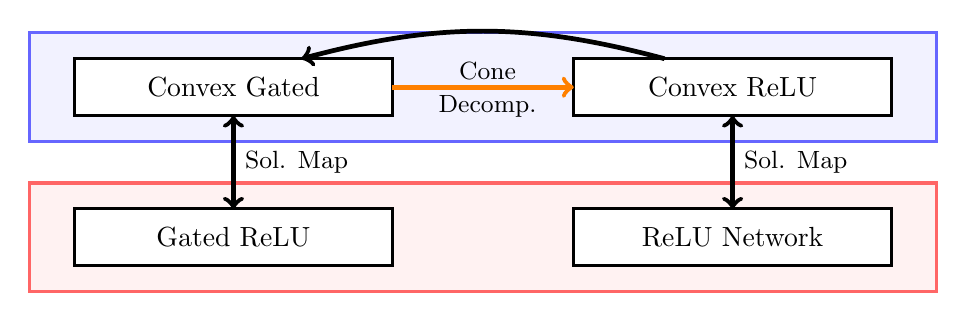
\begin{tikzpicture}[scale=1,
    ]
    \begin{axis}[width=1.1\linewidth, height=5cm,
            axis lines=none,  % don't print axis lines
            yticklabels={,,}, xticklabels={,,},
            ymin=-0.2, ymax=10.2, x axis line style={-},
            xmin=-0.2, xmax=20.2, y axis line style={-},
        ]

        \filldraw[color=blue!60, fill=blue!5, line width=0.4mm](axis cs:0,5.8) rectangle (axis cs:20, 10);
        \filldraw[color=red!60, fill=red!5, line width=0.4mm](axis cs:0,0) rectangle (axis cs:20, 4.2);

        % non-convex models
        \filldraw[line width=0.4mm, fill=white](axis cs:1,1) rectangle (axis cs:8, 3.2) node[pos=.5] {Gated ReLU};
        \filldraw[line width=0.4mm, fill=white](axis cs:12,1) rectangle (axis cs:19, 3.2) node[pos=.5] {ReLU Network};

        % convex models
        \filldraw[line width=0.4mm, fill=white](axis cs:1,6.8) rectangle (axis cs:8, 9) node[pos=.5] {Convex Gated};
        \filldraw[line width=0.4mm, fill=white](axis cs:12,6.8) rectangle (axis cs:19, 9) node[pos=.5] {Convex ReLU};

        \draw [<->, solid, draw=black, line width = 0.6mm] (axis cs:4.5,3.2) -- (axis cs:4.5,6.8) node[right, pos=0.5] {\small Sol. Map};

        \draw [<->, solid, draw=black, line width = 0.6mm] (axis cs:15.5,3.2) -- (axis cs:15.5,6.8)  node[right, pos=0.5] {\small Sol. Map};

        \draw [<-, solid, draw=black, line width = 0.6mm] (axis cs:6,9) to [bend left=15] (axis cs:14, 9);

        \draw [->, solid, draw=orange, line width = 0.6mm] (axis cs:8,7.9) -- (axis cs:12,7.9);
        \node[align=center] at (axis cs:10.1, 7.8) {\small Cone\\ \small Decomp.};
    \end{axis}

\end{tikzpicture}%

%        \else
%            \Huge Relations Figure
%        \fi
%    \end{figure}

%\end{frame}

\begin{frame}{Fast Training: Solving the Convex Programs}
    We develop two algorithms for solving the convex reformulations:

    \vspace{1em}
    \pause

    \begin{itemize}
        \item \textbf{R-FISTA}: a restarted FISTA variant for Gated ReLU.
              \vspace{0.5em}
              \pause
        \item \textbf{AL}: an augmented Lagrangian method for the (constrained) ReLU Problem.
    \end{itemize}

    \pause
    \horizontalrule

    And we can use all the convex tricks!
    \vspace{1em}
    \pause
    \begin{itemize}
        \item \textbf{Fast}: \( O(1/T^2) \) convergence rate using \good{acceleration}.
              \vspace{0.5em}
              \pause

        \item \textbf{Tuning-free}: \good{line-search}, restarts, data normalization, \ldots
              \vspace{0.5em}
              \pause

        \item \textbf{Certificates}: \good{termination} based on min-norm subgradient.
    \end{itemize}

\end{frame}

\begin{frame}{Fast Training: Optimization Performance}

    We generate a performance profile using 438 training problems from the UCI repo.
    \pause

    \begin{figure}[t]
        \centering
        \includegraphics[width=1\linewidth]{assets/pp_main.pdf}
    \end{figure}

    \pause

    \begin{itemize}
        \item R-FISTA/AL solve more, faster, than SGD and Adam.
    \end{itemize}
\end{frame}

\setbeamercolor{background canvas}{bg=LightCyan}
\begin{frame}{}
    \begin{center}
        \huge
        4. Convex Reformulations for Theory of Neural Networks
    \end{center}
\end{frame}
\setbeamercolor{background canvas}{bg=white}

\begin{frame}{Optimal Sets: Summary}
    \begin{center}
        \citep{mishkin2023optimal} Optimal Sets and Solution Paths of {ReLU} Networks.
        \good{A. Mishkin}, M. Pilanci. ICML 2023
    \end{center}

    \horizontalrule
    \pause

    \textbf{Big Idea}: use convex reformulations as an \underline{analytical tool}
    to understand the set of all minimizers for two-layer ReLU networks,
    \vspace{2ex}

    \textbf{Non-Convex Solution Set (NC-ReLU)}:
    \[
        \begin{aligned}
            \calO^*(\lambda)
             & := \argmin_{W_1, w_2} \, \, \half \norm{\sum_{j=1}^m (X W_{1j})_+ w_{2j} - y}_2^2 \\
             & \hspace{6em} + \lambda \sum_{j=1}^m \norm{W_{1j}}_2^2 + |w_{2j}|^2,
        \end{aligned}
    \]

    %\begin{enumerate}
    %    \item \pause
    %          Characterize solutions to the \good{convex reformulation}
    %          using strong duality and KKT conditions.
    %          \vspace{1ex}
    %          \pause
    %    \item Extend results to \bad{non-convex} ReLU networks
    %          using the solution mapping.
    %          \vspace{1ex}
    %          \pause
    %    \item Leverage explicit characterization of the optimal
    %          set for \good{new insights and algorithms}.
    %          \vspace{1ex}
    %          \pause
    %\end{enumerate}

\end{frame}

%\begin{frame}{Optimal Set: Motivation}

%    \textbf{C-ReLU Solution Set}:
%    \[
%        \begin{aligned}
%            \solfn(\lambda) & =
%            \argmin_{v_i, w_i \in \calK_i} \, \bigg\{
%            \half \bigg\|\sum_{D_i \in \tilde \calD} D_i X (v_i - w_i), y\bigg\|_2^2                    \\
%                            & \quad \quad + \lambda\sum_{D_i \in \tilde \calD}\norm{v_i}_2+\norm{w_i}_2
%            \bigg\}.
%        \end{aligned}
%    \]

%    \pause
%    \vspace{0.5ex}
%    \horizontalrule

%    Why care about \( \solfn \)?

%    \pause
%    \vspace{1ex}

%    \begin{itemize}
%        \item \textbf{Generalization}: Different optimal networks can perform
%              differently at \good{test time}.
%              \pause
%              \vspace{1ex}

%        \item \textbf{Compression}: Some optimal models may be \good{smaller than
%                  others}.
%              \pause
%              \vspace{1ex}

%        \item \textbf{Stability}: necessary to understand \good{sensitivity to
%                  perturbations}, \( \solfn(\lambda + \epsilon) \).
%    \end{itemize}

%\end{frame}

\begin{frame}{Optimal Set: Strong Duality}

    \textbf{Convex Reformulation Solution Set (C-ReLU)}:
    \[
        \begin{aligned}
            \solfn(\lambda) & =
            \argmin_{v_i, w_i \in \calK_i} \, \bigg\{
            \half \bigg\|\sum_{D_i \in \tilde \calD} D_i X (v_i - w_i), y\bigg\|_2^2                    \\
                            & \quad \quad + \lambda\sum_{D_i \in \tilde \calD}\norm{v_i}_2+\norm{w_i}_2
            \bigg\}.
        \end{aligned}
    \]

    \pause
    \vspace{0.5ex}
    \horizontalrule

    \textbf{Approach:}

    \pause
    \vspace{1ex}

    \begin{enumerate}
        \item Convex objective + linear constraints \( \implies \) \good{strong duality}!
              \pause
              \vspace{1ex}

        \item We compute the optimal set using the \good{KKT conditions}.
              \pause
              \vspace{1ex}

        \item We then map back onto the \bad{non-convex parameterization}.
              \pause
              \vspace{1ex}

              \begin{itemize}
                  \item A little care is required to handle \bad{model symmetries}.
              \end{itemize}
    \end{enumerate}

    %This recipe applies to other variational properties including
    %\good{uniqueness}, continuity of the \good{regularization path},
    %\good{stability}, etc.

\end{frame}

\begin{frame}{Optimal Set: Characterization}
    \vspace{-2ex}
    \begin{itemize}
        \item
              \textbf{Optimal Fit:}
              \( \hat y := f_{\theta^*}(X) = \sum_{j=1}^m (X W_{1j}^*)_+ w_{2j}^*  \).
              \pause
              \vspace{0.5ex}

        \item
              \textbf{Block Correlations:} A collection of unique
              vectors \( q_i \), with one per activation pattern \( D_i \).
    \end{itemize}

    \vspace{-1ex}
    \pause
    \horizontalrule
    \vspace{-1ex}

    \begin{beamercolorbox}[wd=\textwidth,sep=1em]{result}
        \textbf{Theorem 4.1} \citep{mishkin2023optimal}
        Suppose \( m \geq m^* \).
        Then the optimal set for NC-ReLU up to
        \bad{permutation/split symmetries} is
        \vspace{-1ex}
        \begin{equation*}
            \begin{aligned}
                \hspace{-0.5em} \calO^*(\lambda)  = \,
                \big\{
                 & (W_1,  w_2) :
                \, \textcolor{brightpink}{f_{W_1, w_2}(X) = \hat y}, \\
                 & \forall \, \bi  \in  \calS_\lambda,
                \good{W_{1i} = (\sfrac{\alpha_{i}}{\lambda})^{\sfrac{1}{2}} q_i},
                \good{w_{2i} = (\alpha_i \lambda)^{\sfrac{1}{2}}},
                \alpha_i \geq 0                                      \\
                 & \forall \, \bi  \in [2p] \setminus \calS_\lambda,
                W_{1i} = 0, \, w_{2i} = 0
                \big\}.
            \end{aligned}
        \end{equation*}
        \vspace{-2ex}
    \end{beamercolorbox}
    \pause

    \begin{itemize}
        \item All optimal models have the same fit:
              \textcolor{brightpink}{\( f_{W_1, w_2}(X) = \hat{y} \)}.
              \pause
              \vspace{0.5ex}

        \item The neuron directions are unique:
              \good{\(
                  \frac{W_{1i}^*}{\norm{W_{1i}^*}_2} = q_i / \lambda_i.
                  \)}
    \end{itemize}

\end{frame}

\begin{frame}{Optimal Set: Appearance of Solutions}
    \begin{figure}[]
        \centering
        \includegraphics[width=0.96\textwidth]{assets/solution_sets_vis_270.png}
    \end{figure}

    The non-convex parameterization maps a \good{convex polytope} of
    solutions into a \bad{curved manifold}.

\end{frame}

\begin{frame}{Optimal Set: Exploration and Generalization}
    \begin{itemize}
        \item Take 10,000 samples from the set of optimal neural networks.
              \pause
        \item All samples have (i) \textbf{same training accuracy},
              (ii)~\textbf{same model norm}, but can \bad{generalize differently}.
              \pause
    \end{itemize}

    \begin{figure}[t]
        \centering
        \includegraphics[width=0.48\linewidth]{assets/dist_paper_monks-1.pdf}
        \includegraphics[width=0.48\linewidth]{assets/dist_paper_planning.pdf}
    \end{figure}

    \pause
    The solution you pick (\good{implicit regularization}) is crucial to
    good test performance!

\end{frame}

\begin{frame}{Optimal Set: Comparison to SGD/Adam}
    Fix \( \lambda = 10^{-5} \) and run SGD/Adam \( 1000 \) times
    with \textbf{independent initializations}.
    \pause

    \begin{figure}[t]
        \centering
        \includegraphics[width=0.48\linewidth]{assets/nc_comparison_monks-1.pdf}
        \includegraphics[width=0.48\linewidth]{assets/nc_comparison_planning.pdf}
    \end{figure}

    \pause
    \textbf{Note}: SGD/Adam can converge to \bad{local minima} which may
    perform better in this low-regularization setting.

\end{frame}

\begin{frame}{Neuron Pruning: Minimal Models}
    \textbf{Definition}: An optimal model is \good{minimal} if there
    does not exist another optimal model using a strict subset of active
    neurons.

    \vspace{1ex}
    \pause

    \begin{columns}
        \column{0.5\textwidth}
        \vspace{-1ex}
        \begin{figure}
            \centering
            \includegraphics[width=0.7\textwidth]{assets/polytope.png}
        \end{figure}

        \column{0.5\textwidth}
        \textbf{We prove}:
        \pause
        \begin{itemize}
            \item \good{Vertices} of the C-ReLU optimal set correspond exactly to minimal
                  models.
                  \pause
                  \vspace{1ex}

            \item There are at most \good{\( n \) neurons} in a minimal model.
                  \pause
                  \vspace{1ex}

            \item The \good{smallest minimal model} has exactly \( m^* \) neurons.
                  \begin{itemize}
                      \item \( m^* \iff \) minimum width for convex reformulation.
                  \end{itemize}
        \end{itemize}
    \end{columns}
    \pause
    \vspace{1.5ex}

    We also give a \good{poly-time algorithm} for computing minimal models.
    \vspace{0.5ex}
    \pause

    \hspace{1em} \( \hookrightarrow \) This is the first \underline{optimal pruning
        algorithm} for neural nets!

\end{frame}

\begin{frame}{Neuron Pruning: Performance on UCI Datasets}

    We also show how \textbf{optimal pruning} can be adapted to prune past \(
    m^* \) using a simple \good{correction step} (details in bonus!).

    \pause

    \begin{figure}[t]
        \centering
        \includegraphics[width=0.75\textwidth]{assets/uci_pruning_full_paper.pdf}
    \end{figure}
\end{frame}

\setbeamercolor{background canvas}{bg=LightCyan}
\begin{frame}{}
    \begin{center}
        \huge
        5. Extensions
    \end{center}
\end{frame}
\setbeamercolor{background canvas}{bg=white}

\begin{frame}{Extensions: Scalar Inputs}
    \begin{center}
        \citep{zeger2024library} A Library of Mirrors: Deep Neural Nets in
        Low Dimensions are Convex Lasso Models with Reflection Features. E.
        Zeger, Y. Wang, \good{A. Mishkin}, T. Ergen, E. Cand{\`{e}}s, M.
        Pilanci. SIMODS (\red{In Review}).
    \end{center}

    \horizontalrule
    \pause

    \textbf{Big Idea}: ReLU networks with one-dimensional inputs admit a
    simpler convex reformulation as \good{Lasso models}.
    \pause
    \vspace{1ex}

    \begin{itemize}
        \item The \good{feature matrix} for the Lasso model is
              determined by the model architecture.
              \pause
              \vspace{1ex}

        \item We extend our characterization of the set of \good{optimal ReLU
                  neural networks} to this setting.
    \end{itemize}
\end{frame}

\begin{frame}{Extensions: Mode Connectivity}
    \begin{center}
        \citep{kim2025exploring}
        Exploring The Loss Landscape Of Regularized Neural Networks Via Convex
        Duality. S. Kim, \good{A.  Mishkin}, M. Pilanci. ICLR 2025
        (\red{Oral}).
    \end{center}

    \horizontalrule
    \pause

    \textbf{Mode Connectivity}: how and when are optimal ReLU
    networks connected to each other in weight space?
    \pause
    \vspace{1ex}
    \begin{itemize}
        \item Our previous work assumed \( \bad{m \geq p} \): the
              width of the ReLU network is at least the number of activation
              patterns.
              \pause
              \vspace{1ex}
        \item Now we study the optimal set as \( m \) ranges from \( m^* \)
              to \( p \), creating a set of \good{transitions in connectivity}.
              %\pause
              %\vspace{1ex}

              %\item We also extend our optimal set results to \good{deep linear networks}
              %      and ReLU networks with \good{vector outputs}.
    \end{itemize}
\end{frame}

\begin{frame}{Mode Connectivity: Staircase of Connectivity}

    \begin{beamercolorbox}[wd=\textwidth,sep=1em]{result}
        \textbf{Theorem 2} \citep{kim2025exploring}:
        The critical widths \( m^* \) and \( M^* \) determine connectivity of
        the solution set:
        \pause
        \begin{enumerate}
            \item \( m = m^* \): the optimal set is a finite, \bad{fully
                      disconnected} set.
                  \pause

            \item \( m \geq m^* + 1 \): there exist at least \good{two solutions}
                  which are connected.
                  \pause

            \item  \( m = M^* \): there exists at least \bad{one disconnected
                      solution}.
                  \pause

            \item  \( m \geq M^* + 1\): \good{permutations} of each solution are connected.
                  There are no disconnected points.
                  \pause

            \item \( m \geq \min\cbr{n + 1, m^* + M^*} \): the optimal set is
                  \good{fully connected}.
                  \pause
        \end{enumerate}
    \end{beamercolorbox}
    \pause

    \begin{itemize}
        \item \textbf{Credit}: this theorem is due to Sungyoon Kim,
              building off of my optimal set work with Mert.
    \end{itemize}
\end{frame}

\begin{frame}{Mode Connectivity: Staircase in Action}
    \begin{center}
        \Large
        Staircase of Connectivity Visualized
    \end{center}
    \begin{figure}
        \centering
        \includegraphics[width=0.9\textwidth]{assets/staircase.png}
    \end{figure}
    \pause
    \vspace{2ex}

    \textbf{Takeaway}: Connectivity increases in phases with network width.
    \vspace{1ex}
    \pause

    \hspace{1em} \( \hookrightarrow \) This \good{definitively answers} a long
    standing question in the\\
    \hspace{2.5em} theory of neural networks!

\end{frame}

\begin{frame}{Extensions: Feature-Sparse Neural Networks}
    \begin{center}
        Convex LassoNet: Feature Sparse Convex Reformulations.
        \good{A.  Mishkin}, T. Ergen, F. Ruan, M. Pilanci, R. Tibshirani.
        (\red{Ongoing})
    \end{center}

    \horizontalrule
    \pause

    \textbf{Big Idea}: combine feature-sparsity with global optimization
    to \underline{improve generalization}.

    \pause
    \vspace{1ex}

    \begin{itemize}
        \item Naive approaches to feature sparsity in ReLU networks using group
              norms \bad{underperform} \citep{feng2017sparse}.
              \pause
              \vspace{0.5ex}

        \item But sophistical approaches like LassoNet
              \citep{lemhadri2021lassonet} are hard to train and can get
              trapped in \bad{local minima}.
              \pause
              \vspace{0.5ex}

        \item We derive \good{sparsity-inducing} convex reformulations with
              \good{global optimization} guarantees.
    \end{itemize}

\end{frame}

\begin{frame}{Feature-Sparsity: Planted Neural Networks}

    \begin{figure}
        \centering
        \includegraphics[width=0.75\textwidth]{assets/mip_relu_nn_100.pdf}
    \end{figure}

\end{frame}

\begin{frame}{Feature-Sparsity: Real Data}
    \begin{figure}
        \centering
        \includegraphics[width=0.75\textwidth]{assets/uci_regression_150.pdf}
    \end{figure}
\end{frame}

\begin{frame}{Extensions: Convexifying Deep Networks}
    \begin{center}
        Deep Convex Reformulations: Equivalences and Optimal Sets. \good{A.
            Mishkin}, M. Pilanci. (\red{Ongoing Work})
    \end{center}

    \horizontalrule
    \pause

    \textbf{Big Idea}: Extend convex reformulations to \good{deep ReLU
        networks} without relying on \bad{restricted architectures}.

    \pause
    \vspace{1ex}

    \begin{itemize}
        \item Three layer networks have \bad{non-linear}
              combinations of \bad{non-linear} functions, which are challenging
              to analyze.
              \pause
              \vspace{0.5ex}

        \item But, once we understand \good{three layer} networks, we understand
              \good{\( k \)-layer} networks for any \( k \geq 1 \).
              \pause
              \vspace{0.5ex}

        \item  We prove that ReLU MLPs of arbitrary depth are \good{convex
                  functions} with non-convex \bad{tensor decomposition} constraints.

    \end{itemize}

\end{frame}

\begin{frame}{Deep Networks: Layer Elimination}

    Let \( W^{(l)} \in \R^{d_{l-1} \times d_l} \) and
    consider the \( k \)-layer ReLU network
    \[
        f_\theta(X) = \rbr{\rbr{\rbr{X W^{(1)}}_+ W^{(2)}}_+ W^{(3)} \cdots }_+ W^{(k)}.
    \]

    \pause
    \horizontalrule

    \textbf{Question}: how do we construct a \good{convex reformulation}?

    \pause
    \vspace{1ex}

    \begin{enumerate}
        \item The first \good{two-layer block} has a convex reformulation in
              terms of the activation patterns \( D_i \),
              \[
                  f_\theta(X) = \rbr{\rbr{\sum_{i=1}^p D_i X T_i^{(2)} }_+ \otimes W_i^{(3)} \cdots }_+ W^{(k)}.
              \]
              \pause
              \vspace{0.5ex}

        \item This creates another \good{two-layer block}, which has a convex
              reformulation in terms of the activation patterns \( D_j^{(2)} \)\ldots
    \end{enumerate}

\end{frame}

\begin{frame}{Deep Networks: Tensor Programs}

    Let \( T^{(l)} \in \R^{d_0 \times \ldots d_{l}} \) be a tensor with
    low-rank decomposition,
    \[
        T^{(l)} \in \calG^{(l)} \approx \cbr{ T^{(l)} :
        \exists \, T^{(l-1)} \in \calG^{(l-1)} \text{ s.t. }
        T^{l}_i = T_i^{(l-1)} \otimes W^{(l)}_i.
        }
    \]
    \vspace{-3ex}
    \pause

    \begin{beamercolorbox}[wd=\textwidth,sep=1em]{result}
        \textbf{Proposition}:
        Training a \( k \)-layer ReLU model,
        \begin{equation*}
            \min_{\theta} \calL\rbr{f_{\theta}(X), y},
        \end{equation*}
        is equivalent to solving the order \( k+1 \) tensor program
        \begin{equation*}
            \min_{T^{(k)}} \, \calL\rbr{X^{(k)} \odot T^{(k)}, y}
            \quad \text{s.t.} \quad T^{(k)} \in \calG^{(k)}.
        \end{equation*}
        \vspace{-4ex}
    \end{beamercolorbox}
    \pause

    \begin{itemize}
        \item \( \text{rank}(T^{(k)}) \leq d_0 \prod_{l=1}^k b_l \),
              where \( b_l \leq d_l \) is the number of \good{unique activation
                  patterns} occurring in layer \( l \).
              \pause
              \vspace{0.5ex}

        \item If \( d_l \geq 2 p_l d_{l+1} \) for every \( l \), then this
              becomes \good{fully convex}.
    \end{itemize}

\end{frame}

\begin{frame}{Deep Networks: Tensor Parameterization}

    \textbf{Q}: What does the tensor \( T \) represent?
    \pause
    \vspace{1ex}

    \textbf{A}: Each entry \( T_{i_0, i_1, \ldots, i_{k}} \) is a
    path through the network DAG.
    \pause

    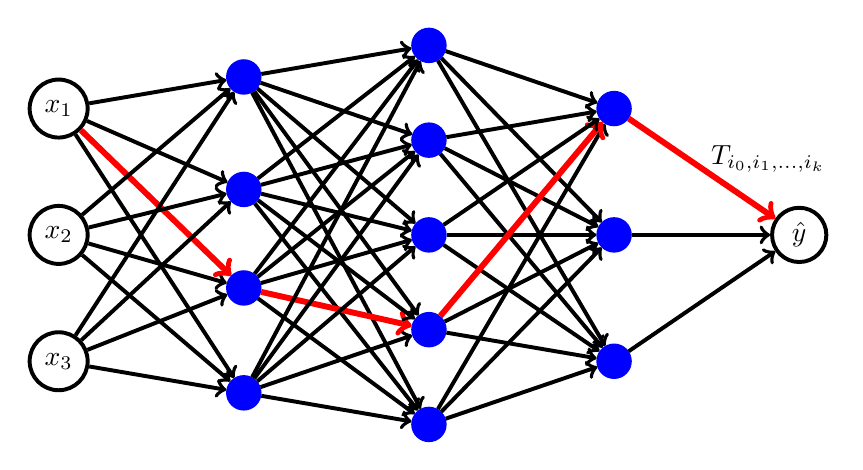
\begin{tikzpicture}[scale=1,
    ]
    \begin{axis}[width=1.1\textwidth, height=8cm,
            axis lines=none,  % don't print axis lines
            yticklabels={,,}, xticklabels={,,},
            ymin=0, ymax=8, y axis line style={-},
            xmin=0, xmax=15, x axis line style={-},
        ]
        %\node [] (input) at (axis cs:1,4) {$X$};
        \node [Input] (input1) at (axis cs:2,2) {$x_3$};
        \node [Input] (input2) at (axis cs:2,4) {$x_2$};
        \node [Input] (input3) at (axis cs:2,6) {$x_1$};

        %\draw [decorate, line width = 0.6mm,
        %    decoration = {calligraphic brace}] (axis cs:2,1.5) --  (axis cs:2,6.5);

        \node [Hidden] (hidden11) at (axis cs:5,1.5) {};
        \node [Hidden] (hidden12) at (axis cs:5,3.16) {};
        \node [Hidden] (hidden13) at (axis cs:5,4.72) {};
        \node [Hidden] (hidden14) at (axis cs:5,6.5) {};

        \node [Hidden] (hidden21) at (axis cs:8,1) {};
        \node [Hidden] (hidden22) at (axis cs:8,2.5) {};
        \node [Hidden] (hidden23) at (axis cs:8,4) {};
        \node [Hidden] (hidden24) at (axis cs:8,5.5) {};
        \node [Hidden] (hidden25) at (axis cs:8,7) {};

        \node [Hidden] (hidden31) at (axis cs:11,2) {};
        \node [Hidden] (hidden32) at (axis cs:11,4) {};
        \node [Hidden] (hidden33) at (axis cs:11,6) {};

        \node [Output] (output) at (axis cs:14,4) {$\hat y$};

        % Layer 1

        \draw [->, style=arrow, draw=black] (input1) -- (hidden11);
        \draw [->, style=arrow, draw=black] (input2) -- (hidden11);
        \draw [->, style=arrow, draw=black] (input3) -- (hidden11);

        \draw [->, style=arrow, draw=black] (input1) -- (hidden12);
        \draw [->, style=arrow, draw=black] (input2) -- (hidden12);
        \draw [->, style=arrow, draw=red, line width = 0.75mm] (input3) -- (hidden12);

        \draw [->, style=arrow, draw=black] (input1) -- (hidden13);
        \draw [->, style=arrow, draw=black] (input2) -- (hidden13);
        \draw [->, style=arrow, draw=black] (input3) -- (hidden13);

        \draw [->, style=arrow, draw=black] (input1) -- (hidden14);
        \draw [->, style=arrow, draw=black] (input2) -- (hidden14);
        \draw [->, style=arrow, draw=black] (input3) -- (hidden14);

        % Layer 2

        \draw [->, style=arrow, draw=black] (hidden11) -- (hidden21);
        \draw [->, style=arrow, draw=black] (hidden12) -- (hidden21);
        \draw [->, style=arrow, draw=black] (hidden13) -- (hidden21);
        \draw [->, style=arrow, draw=black] (hidden14) -- (hidden21);

        \draw [->, style=arrow, draw=black] (hidden11) -- (hidden22);
        \draw [->, style=arrow, draw=red, line width = 0.75mm] (hidden12) -- (hidden22);
        \draw [->, style=arrow, draw=black] (hidden13) -- (hidden22);
        \draw [->, style=arrow, draw=black] (hidden14) -- (hidden22);

        \draw [->, style=arrow, draw=black] (hidden11) -- (hidden23);
        \draw [->, style=arrow, draw=black] (hidden12) -- (hidden23);
        \draw [->, style=arrow, draw=black] (hidden13) -- (hidden23);
        \draw [->, style=arrow, draw=black] (hidden14) -- (hidden23);

        \draw [->, style=arrow, draw=black] (hidden11) -- (hidden24);
        \draw [->, style=arrow, draw=black] (hidden12) -- (hidden24);
        \draw [->, style=arrow, draw=black] (hidden13) -- (hidden24);
        \draw [->, style=arrow, draw=black] (hidden14) -- (hidden24);

        \draw [->, style=arrow, draw=black] (hidden11) -- (hidden25);
        \draw [->, style=arrow, draw=black] (hidden12) -- (hidden25);
        \draw [->, style=arrow, draw=black] (hidden13) -- (hidden25);
        \draw [->, style=arrow, draw=black] (hidden14) -- (hidden25);

        % Layer 3

        \draw [->, style=arrow, draw=black] (hidden21) -- (hidden31);
        \draw [->, style=arrow, draw=black] (hidden22) -- (hidden31);
        \draw [->, style=arrow, draw=black] (hidden23) -- (hidden31);
        \draw [->, style=arrow, draw=black] (hidden24) -- (hidden31);
        \draw [->, style=arrow, draw=black] (hidden25) -- (hidden31);

        \draw [->, style=arrow, draw=black] (hidden21) -- (hidden32);
        \draw [->, style=arrow, draw=black] (hidden22) -- (hidden32);
        \draw [->, style=arrow, draw=black] (hidden23) -- (hidden32);
        \draw [->, style=arrow, draw=black] (hidden24) -- (hidden32);
        \draw [->, style=arrow, draw=black] (hidden25) -- (hidden32);

        \draw [->, style=arrow, draw=black] (hidden21) -- (hidden33);
        \draw [->, style=arrow, draw=red, line width = 0.75mm] (hidden22) -- (hidden33);
        \draw [->, style=arrow, draw=black] (hidden23) -- (hidden33);
        \draw [->, style=arrow, draw=black] (hidden24) -- (hidden33);
        \draw [->, style=arrow, draw=black] (hidden25) -- (hidden33);

        \draw [->, style=arrow, draw=black] (hidden31) -- (output);
        \draw [->, style=arrow, draw=black] (hidden32) -- (output);
        \draw [->, style=arrow, draw=red, line width = 0.75mm] (hidden33) -- (output) node[pos=0.4,right] {\hspace{0.2ex} $T_{i_0, i_1, \ldots, i_k}$};

        %\draw [->, style=arrow, draw=black] (hidden4) -- (output) node[pos=0.5,above] {$w_{2j}$};
    \end{axis}

\end{tikzpicture}%


\end{frame}

\setbeamercolor{background canvas}{bg=LightCyan}

\begin{frame}{}
    \begin{center}
        \huge Big-Picture Summary
    \end{center}
\end{frame}
\setbeamercolor{background canvas}{bg=white}

\begin{frame}{Big-Picture Summary}

    \textbf{Summary}: We use convex reformulations for breakthroughs
    in training and neural network theory.
    \vspace{1ex}
    \pause
    \begin{itemize}
        \item \textbf{Fast Training}:
              We develop two fast, \good{tuning-free algorithms} to train (or
              approximate) two-layer ReLU networks.

              \pause
              \vspace{1ex}

        \item \textbf{Optimal Sets}:
              We characterize all \good{global optima} for training
              two-layer ReLU networks.
              \pause
              \vspace{1ex}

        \item \textbf{Deep Networks}:
              We show that that deep ReLU networks are \good{tensor programs}
              that convexify with increasing width.
              \pause
              \vspace{1ex}

        \item \textbf{Additional Results}:
              We provide many, many more results on \good{continuity},
              \good{stability}, \good{optimization}, and other areas.
    \end{itemize}

\end{frame}

\begin{frame}{Overview: Publications and Ongoing Projects}

    \textbf{Publications}:

    {\small
    \begin{enumerate}
        \item Fast Convex Optimization for Two-Layer ReLU Networks. \good{A.
                  Mishkin}, A. Sahiner, M. Pilanci. ICML 2022.

        \item Optimal Sets and Solution Paths of {ReLU} Networks. \good{A.
                  Mishkin}, M. Pilanci. ICML 2023.

        \item A Library of Mirrors: Deep Neural Nets in Low Dimensions are
              Convex Lasso Models with Reflection Features. E. Zeger, Y. Wang,
              \good{A. Mishkin}, T. Ergen, E. Cand{\`{e}}s, M. Pilanci. SIMODS
              (\red{In Review}).

        \item Exploring The Loss Landscape Of Regularized Neural Networks Via
              Convex Duality. S. Kim, \good{A.  Mishkin}, M. Pilanci. ICLR 2025
              (\red{Oral}).
    \end{enumerate}
    }

    \textbf{Ongoing Projects}:
    { \small
    \begin{enumerate}
        \item Deep Convex Reformulations: Equivalences and Optimal Sets

        \item Convex LassoNet: Feature-Sparse Convex Reformulations
    \end{enumerate}
    }

\end{frame}

\begin{frame}{Overview: Additional Projects (\red{Details in Bonus})}

    \textbf{Additional Publications}:
    {\small
    \begin{enumerate}
        \item Directional Smoothness and Gradient Methods: Convergence and
              Adaptivity. \good{A. Mishkin}*, A. Khaled*, Y. Wang, A. Defazio, R. M.
              Gower. NeurIPS 2024.

        \item  Level Set Teleportation: An Optimization Perspective. \good{A.
                  Mishkin}, A. Bietti, R. M. Gower. AISTATS 2025.

        \item Glocal Smoothness: Line Search can really help! C. Fox, \good{A.
                  Mishkin}, S. Vaswani, M. Schmidt. SIOPT (\red{In Review}).
    \end{enumerate}
    }

    \textbf{Further Ongoing Projects}:

    { \small
    \begin{enumerate}
        \item Greedy 2-Coordinate Updates for
              Equality-Constrained Optimization via Steepest Descent in the
              1-Norm. A. V. Ramesh*, \good{A. Mishkin}*, M. Schmidt, Y. Zhou, J.
              Lavington, J. She. (\red{To Be Submitted})

        \item Global Convergence of Gradient Flow on 1D Data with Sign Noise.
              \good{A. Mishkin}, F. Bach.
    \end{enumerate}
    }
\end{frame}

\begin{frame}{Acknowledgements}

    My PhD has benefited from collaborations with many \good{mentors}, friends,
    and fellow students. Many thanks to,
    \vspace{1ex}
    \pause

    \begin{itemize}
        \item \textbf{Stanford}: \underline{\good{Mert Pilanci}},
              Sungyoon Kim, Tolga Ergen (LG AI), Arda Sahiner (Arcus), Emi
              Zeger, and many others.
              \pause
              \vspace{1ex}

        \item \textbf{Voleon}: \good{Sahand Negahban}, \good{Deepak Rajan},
              Alex Appleton.
              \pause
              \vspace{1ex}

        \item \textbf{Inria Paris}: \good{Francis Bach}, Frederik Kunstner.
              \pause
              \vspace{1ex}

        \item \textbf{The Flatiron Institute}:  \good{Alberto Bietti},
              \good{Robert Gower}, Aaron Defazio (Meta FAIR), Ahmed Khaled
              (Princeton), Yuanhao Wang (Princeton).
              \pause
              \vspace{1ex}

        \item \textbf{UBC}: \good{Mark Schmidt}, Jonathan Lavington (Amazon),
              Si Yi Meng (Cornell), Sharan Vaswani (SFU).
              \pause
              \vspace{1ex}

        \item \textbf{RIKEN AIP}: \good{Emtiyaz Khan}, Didrik Nielsen (Twig).
    \end{itemize}

\end{frame}

\begin{frame}{Acknowledgements Continued}

    Lastly, I want to make special mention of the following people:

    \pause
    \vspace{1ex}

    \begin{itemize}
        \item \good{My committee members}: Mert Pilanci, Stepehn Boyd, Mykel
              Kochenderfer, Balaji Prabhakar, Aaron Sidford, and Robert
              Tibshirani.
              \pause
              \vspace{1ex}

        \item My partner, \good{Sophie Boerlage}, for believing in me
              throughout this long journey.
              \pause
              \vspace{1ex}

        \item \good{Frederik Kunstner}, without whom I probably wouldn't have
              stumbled into optimization.
              \pause
              \vspace{1ex}

        \item And, of course, my \good{family}, whose constant support made
              all of this possible.
    \end{itemize}

\end{frame}

%% main content ends %%

%% bibliography
\begin{frame}[allowframebreaks]{References}
    \printbibliography[]
\end{frame}

%!TEX root = ../main.tex

\setbeamercolor{background canvas}{bg=LightCyan}
\begin{frame}{}
    \begin{center}
        \huge Additional Projects
    \end{center}
\end{frame}
\setbeamercolor{background canvas}{bg=white}

\begin{frame}{Directional Smoothness: Summary}
    \citep{mishkin2024directional}
    Directional Smoothness and Gradient Methods: Convergence and Adaptivity.
    \good{A. Mishkin}*, A. Khaled*, Y. Wang, A. Defazio, R. M.  Gower. NeurIPS
    2024.

    \horizontalrule

    \pause
    \textbf{Big Idea}: GD is a local algorithm, so the analysis should be
    local.
    \vspace{1ex}

    \pause
    \textbf{Main Contributions}:
    \pause
    \vspace{0.5ex}
    \begin{itemize}
        \item \good{Directional Smoothness}: concrete functions \( M(x, y) \)
              that measure the Lipschitz smoothness of \( f \) between \( x \)
              and \( y \).
              \pause
              \vspace{1ex}

        \item \good{Path-Dependent Rates}: Convergence bounds for gradient descent
              that depend only on \( M(\xkk, \xk) \).
              \pause
              \vspace{1ex}

        \item \good{Adaptive Methods}: algorithms which are ``strongly adaptive''
              to the directional smoothness along the optimization path.
    \end{itemize}
\end{frame}

\begin{frame}{Level Set Teleportation: Summary}
    \citep{mishkin2025level}
    Level Set Teleportation: An Optimization Perspective. \good{A.  Mishkin},
    A. Bietti, R. M. Gower. AISTATS 2025.

    \horizontalrule
    \pause

    \textbf{Big Idea}: rigorously analyze and experimentally evaluate
    Newton-like ``teleportation'' methods \citep{zhao2022symmetry}.

    \vspace{1ex}

    \pause
    \textbf{Main Contributions}:
    \pause
    \vspace{0.5ex}
    \begin{itemize}
        \item \good{Sub-Level Set Teleportation}:
              a co-routine to accelerate optimization by maximizing the gradient
              over a sub-level set,
              \[
                  x_k^+ = \argmin_x \cbr{\norm{\grad(x)}_2 : f(x) \leq f(x_k)}.
              \]
              \pause

        \item We give a novel analysis combining \good{linear progress}
              from teleportation with sub-linear
              rates for non-strongly convex GD.

              \pause
              \vspace{1ex}

        \item We also develop \good{parameter-free algorithms} for solving
              general, non-linear sub-level set teleportation problems in
              practice.
    \end{itemize}
\end{frame}

\begin{frame}{Glocal Smoothness: Summary}
    \citep{fox2025glocal}
    Glocal Smoothness: Line Search can really help! C. Fox, \good{A.  Mishkin},
    S. Vaswani, M. Schmidt. SIOPT (\red{In Review}).

    \horizontalrule

    \pause
    \textbf{Big Question}: Can we show provable speed-ups from line-search?
    \vspace{1ex}

    \pause
    \textbf{Main Contributions}:
    \pause
    \vspace{0.5ex}
    \begin{itemize}
        \item \good{Glocal smoothness}: functions which are globally
              \( L \)-Lipschitz smooth and locally \( L^* \)-smooth
              (\( L^* \ll L \)) around minimizers.
              \pause
              \vspace{1ex}

        \item Convergence rates showing GD with exact line-search and GD with
              the Polyak step-size \good{adapt} to glocal smoothness.

              \pause
              \vspace{1ex}

        \item Extensions to \good{Nesterov acceleration}, with and without
              a backtracking line-search.
    \end{itemize}
\end{frame}

\begin{frame}{Greedy Block-Coordinate Descent: Summary}
    \citep{ramesh2023greedy}
    Greedy 2-Coordinate Updates for Equality-Constrained Optimization via Steepest
    Descent in the 1-Norm. A. V. Ramesh*, \good{A. Mishkin}*, M. Schmidt, et al.
    (\red{To Be Submitted})

    \horizontalrule
    \pause

    \textbf{Problem}: greedy rules out-perform random selection for training
    SVMs, but rates don't reflect this.

    \vspace{1ex}

    \pause
    \textbf{Main Contributions}:
    \pause
    \vspace{0.5ex}
    \begin{itemize}
        \item New analyses of \good{block-coordinate descent} for separable
              optimization problems with linear coupling constraints.
              \pause
              \vspace{1ex}

        \item \good{Single Constraint}: We prove that the GS-q rule
              \citep{tseng2009block} is equivalent to steepest descent in the
              \( \ell_1 \)-norm, leading to fast rates with \( \mu_1 \)
              dependence.

              \pause
              \vspace{1ex}

        \item \good{Multiple Constraints}: We extend the conformal vector
              framework used by \citet{tseng2009block} to obtain rates
              which improve with block-size.
    \end{itemize}
\end{frame}

\begin{frame}{Gradient Flows: Summary}
    Global Convergence of Gradient Flow on 1D Data with Sign Noise.  \good{A.
        Mishkin}, F. Bach. (\red{Ongoing})

    \horizontalrule
    \pause

    \textbf{Big Idea}: understand how ``neuron diversity'' affects convergence
    of the gradient flow for shallow ReLU networks.

    \vspace{1ex}

    \pause
    \textbf{Main Contributions}:
    \pause
    \vspace{0.5ex}
    \begin{itemize}
        \item \good{Diversity}: model neurons have different activation patterns.
              \pause
              \vspace{1ex}

        \item We find diversity is preserved for simple anti-correlated noise
              and the gradient flow is \good{globally convergent}.
              \pause
              \vspace{1ex}

        \item The gradient flow demonstrates \good{saddle-to-saddle dynamics}
              \citep{pesme2023saddle}, with saddles corresponding to model
              complexity.
              \pause
              \vspace{1ex}
    \end{itemize}

    \textbf{Remaining Extensions}:
    \pause
    \begin{enumerate}
        \item Generalize the target noise to more \bad{interesting/realistic}
              regimes (e.g. fractional Brownian motion).
    \end{enumerate}
\end{frame}

\setbeamercolor{background canvas}{bg=LightCyan}
\begin{frame}{}
    \begin{center}
        \huge Background on Convex Neural Networks
    \end{center}
\end{frame}
\setbeamercolor{background canvas}{bg=white}

\begin{frame}{Bonus: Convex Neural Networks}
    \begin{itemize}
        \item Let \( X \in \R^{n \times d} \) be a training matrix and \( y \in \R^n \)
              the targets.
              \vspace{1ex}
              \pause

        \item Let \( f_\theta : \R^n \into \R \) be a neural network with parameters
              \( \theta \).
    \end{itemize}
    \vspace{1ex}
    \pause
    The standard ERM training problem is,
    \[
        \Theta^* = \argmin_{\theta} \sum_{i=1}^n \mathcal{L}(f_\theta(x_i), y_i) + r(\theta),
    \]
    where \( \calL \) is a loss function and \( r \) is a regularizer.
    \pause
    \vspace{1ex}

    \begin{itemize}
        \item \( f_\theta \) is a \good{convex neural network} if this problem
              is convex in \( \theta \).
              \vspace{1ex}
              \pause
        \item This is distinct from \bad{input-convex} neural networks, where
              \( x \mapsto f_\theta(x) \) is convex \citep{amos2017input}.
    \end{itemize}

\end{frame}

\begin{frame}{Bonus: Brief Literature Review}
    There are multiple flavours of convex neural networks:
    \vspace{1ex}

    \begin{itemize}
        \item \citet{bengio2005convex} develop a \good{gradient-boosting algorithm}
              where the problem of adding one neuron at a time is convex.
              \pause
              \vspace{1ex}

        \item \citet{bach2017breaking} study the generalization performance of
              \good{infinite-width} two-layer neural networks (which are convex).
              \pause
              \vspace{1ex}

        \item \citet{pilanci2020convex} develop finite-width \textbf{convex
                  reformulations} for two-layer ReLU networks using \good{duality}.
              \pause
    \end{itemize}
    \vspace{1ex}

    These approaches differ primarily in how they discretize the underlying
    infinite-width neural network.

\end{frame}

\begin{frame}{Bonus: Function Space Viewpoint}
    \citet{bengio2005convex, bach2017breaking} take a function space approach:

    \begin{itemize}
        \item Let \( \sigma \) be an activation function and define
              \[
                  \calH = \cbr{h : w \in \R^d, h(x) = \sigma(x^\top w)}.
              \]
              \pause

        \item Write problem as optimization over function space \( W \):
              \[
                  \min_{w \in \calW} \cbr{\sum_{j=1}^n L\rbr{\sum_{h_i \in \calH} w_i h_i(x_j), y_j} + R(w)}.
              \]

              \pause

        \item If \( R \) is sparsity inducing, then the final network may have finite width.
    \end{itemize}

\end{frame}

\begin{frame}{Bonus: Related Work Cont.}
    \citet{bengio2005convex}: algorithm-focused approach.
    \vspace{1ex}
    \begin{itemize}
        \item Take \( R(w) = \norm{w}_1 \) and \( L(\hat y, y) = \max\cbr{0, 1 - \hat y y} \).
              \pause
              \vspace{1ex}
        \item Show that \( \text{nnz}(w^*) \leq n+1 \), meaning the final model is finite.
              \pause
              \vspace{1ex}
        \item Propose a boosting-type algorithm for iteratively adding neurons.
    \end{itemize}

\end{frame}
\begin{frame}{Bonus: Related Work Cont.}
    \citet{bach2017breaking}: analysis-focused approach.

    \begin{itemize}
        \item Handle spaces/functions properly using measure theory.
              \vspace{1ex}
              \pause
              \begin{itemize}
                  \item \( \calW \) is a space of signed measures, prediction is
                        \[
                            f(x) = \int_{\calH} h(x) dw(h)
                        \]
                        \vspace{1ex}
                        \pause

                  \item \( R \) is weighted total variation of measure \( w \).
                        \pause
                        \vspace{1ex}

                  \item Setup reduces to \citet{bengio2005convex} in finite spaces.
              \end{itemize}

              \pause
              \vspace{1ex}
        \item Guarantee that \( m^* \leq n \) using a representer theorem.
              \pause
              \vspace{1ex}

        \item Derive an incremental algorithm based on Frank-Wolfe, but incremental steps are NP-Hard
              for ReLU activations.
    \end{itemize}

\end{frame}

\begin{frame}{Bonus: Key Representer Theorem}
    \begin{theorem}[\citet{rogosinski1958moments}]
        If \( \rbr{\Omega, \calB} \) is a Borel space, \( \mu \) is a measure,
        \( g_i \), \( i \in \cbr{1, \ldots n} \) are measurable and \( \mu \)-integrable,
        then there exists measure \( \hat \mu \) with finite support at most \( n \)
        such that
        \[
            \int_\Omega g_i(\omega) d\mu(\omega) = \int_\Omega g_i(\omega) d \hat \mu(\omega)
        \]
        for all \( i \in \cbr{1,\ldots,n} \).
    \end{theorem}

    Prediction for dataset with \( n \) dimensions:
    \[
        f(x_i) = \int_{\calH} h(x_i) dw(h) = \sum_{h = 1}^m h_j(x_i) w(h_j),
    \]
    where \( m \leq n \) and \( h_j(x) = \rbr{\abr{x, w_j}}_+ \).
\end{frame}

\setbeamercolor{background canvas}{bg=LightCyan}
\begin{frame}{}
    \begin{center}
        \huge Convex Reformulations
    \end{center}
\end{frame}
\setbeamercolor{background canvas}{bg=white}

\begin{frame}{Convex Reformulations: Breaking it Down}

    \[
        \begin{aligned}
            \min_{u} & \norm{\sum_{j=1}^p D_j X (v_j - w_j) - y}_2^2 +
            \lambda \sum_{j=1}^p \norm{v_j}_2 + \norm{w_j}_2           \\
                     & \hspace{0.2em} \text{s.t. }
            v_j, w_j \in \calK_j := \cbr{w : (2D_j - I) X w \geq 0},
        \end{aligned}
    \]
    where \( \purple{D_j = \text{diag}[\mathbbm{1}(X g_j \geq 0)]} \).

    \horizontalrule

    \begin{itemize}
        \item \purple{\( D_j \) is a ReLU activation pattern induced by ``gate'' \( g_j \).}
              \pause
              \begin{itemize}
                  \item \([D_j]_{ii} = 1\) if \( \abr{x_i, g_i} \geq 0 \) and \( 0 \) otherwise.
              \end{itemize}

    \end{itemize}
    \vspace{7.3em}
\end{frame}

\begin{frame}{Convex Reformulations: Breaking it Down}

    \[
        \begin{aligned}
            \min_{u} & \norm{\sum_{j=1}^p D_j X (v_j - w_j) - y}_2^2 +
            \purple{\lambda \sum_{j=1}^p \norm{v_j}_2 + \norm{w_j}_2}  \\
                     & \hspace{0.2em} \text{s.t. }
            v_j, w_j \in \calK_j := \cbr{w : (2D_j - I) X w \geq 0}
        \end{aligned}
    \]
    where \( D_j = \text{diag}[\mathbbm{1}(X g_j \geq 0)] \).

    \horizontalrule

    \begin{itemize}
        \item \( D_j \) is a ReLU activation pattern induced by ``gate'' \( g_j \).
              \begin{itemize}
                  \item \([D_j]_{ii} = 1\) if \( \abr{x_i, g_i} \geq 0 \) and \( 0 \) otherwise.
              \end{itemize}
        \item \purple{Weight-decay regularization turns into ``group \( \ell_1 \)'' penalty.}
    \end{itemize}
    \vspace{6em}
\end{frame}

\begin{frame}{Convex Reformulations: Breaking it Down}

    \[
        \begin{aligned}
            \min_{u} & \norm{\sum_{j=1}^p D_j X (v_j - w_j) - y}_2^2 +
            \lambda \sum_{j=1}^p \norm{v_j}_2 + \norm{w_j}_2           \\
                     & \hspace{0.2em} \purple{\text{s.t. }
                v_j, w_j \in \calK_j := \cbr{w : (2D_j - I) X w \geq 0},}
        \end{aligned}
    \]
    where \( D_j = \text{diag}[\mathbbm{1}(X g_j \geq 0)] \).

    \horizontalrule

    \begin{itemize}
        \item \( D_j \) is a ReLU activation pattern induced by ``gate'' \( g_j \).
              \begin{itemize}
                  \item \([D_j]_{ii} = 1\) if \( \abr{x_i, g_i} \geq 0 \) and \( 0 \) otherwise.
              \end{itemize}
        \item Weight-decay regularization turns into ``group \( \ell_1 \)'' penalty.
        \item \purple{The constraint \( v_j \in \calK_j \) implies
                  \[
                      \rbr{X v_j}_+ = D_j X v_j.
                  \]
                  That is, \( v_j \) has the activation encoded by \( D_j \).
              }
    \end{itemize}
\end{frame}

\begin{frame}{Bonus: Explicit Solution Mapping}

    Given \( \rbr{v^*, w^*} \), an optimal non-convex ReLU network is given by

    \begin{equation*}
        \textbf{C to NC:} \quad \quad
        \begin{aligned}
            W_{1i} & = v_i^*/ \sqrt{\norm{v_i^*}}, \quad w_{2i} = \sqrt{\norm{v_i^*}}
            \\
            W_{1j} & = w_i^*/ \sqrt{\norm{w_i^*}}, \quad w_{2j} = -\sqrt{\norm{w_i^*}}.
        \end{aligned}
    \end{equation*}

    \begin{itemize}
        \item Optimal solution balances weight between layers.
    \end{itemize}

    \horizontalrule

    Given \( (W^*_{1i}, w^*_{2i}) \), an optimal convex ReLU model is

    \begin{equation*}
        \textbf{NC to C:} \quad \quad
        \begin{aligned}
            v_i & = W^*_{1i} \abs{w_{2i}}^* \quad \text{ if } w^*_{2i} \geq 0 \\
            w_i & = W^*_{1i} \abs{w_{2i}}^* \quad \text{ Otherwise.}
        \end{aligned}
    \end{equation*}

    \begin{itemize}
        \item Optimal solution combines weight from both layers.
    \end{itemize}

\end{frame}

\setbeamercolor{background canvas}{bg=LightCyan}
\begin{frame}{}
    \begin{center}
        \huge Gated ReLU Networks and Cone Decompositions
    \end{center}
\end{frame}
\setbeamercolor{background canvas}{bg=white}

\begin{frame}{Bonus: Gated ReLU Networks}

    \begin{beamercolorbox}[wd=\textwidth,sep=1em]{result}
        \textbf{Theorem 2.2} (informal): C-GReLU is equivalent to solving
        \[
            \textbf{NC-GReLU}: \min_{W_1, \alpha} \half \norm{\sum_{j=1}^p \phi_{g_j}(X, w_{j})\alpha - y}_2^2 + \frac{\lambda}{2} \sum_{j=1}^p \norm{w_{j}}_2^2 + |\alpha_j|^2,
        \]
        with the ``Gated ReLU'' \citep{fiat2019decoupling} activation function
        \[ \phi_{g}(X, u) = \text{diag}(\mathbbm{1}(Xg \geq 0)) X u, \]
        and gate vectors \( g_j \) such that
        \[
            D_j = \text{diag}[\mathbbm{1}(X g_j \geq 0).
        \]
    \end{beamercolorbox}
    \pause

    \textbf{Interpretation}: if \( u_j \not \in \calK_j \), then the activation
    must be decoupled from the linear mapping in the non-convex model.

\end{frame}

\begin{frame}{Bonus: Cone Decompositions}

    \begin{center}
        \textbf{Question}: when are Gated ReLU and ReLU networks equivalent?
    \end{center}

    \pause
    \horizontalrule

    Consider special case where \( \lambda = 0 \).

    \[
        \textbf{C-GReLU}: \min_{u} \norm{\sum_{j=1}^p D_j X u_j - y}_2^2. \hspace{11em}
    \]
    \vspace{-1em}

    \begin{center}
        \Large \red{V.S.}
    \end{center}

    \vspace{-2em}
    \[
        \begin{aligned}
            \textbf{C-ReLU}: \min_{u} & \norm{\sum_{j=1}^p D_j X (v_j - w_j) - y}_2^2. \\
                                      & \hspace{0.2em} \text{s.t. }
            v_j, w_j \in \calK_j := \cbr{w : (2D_j - I) X w \geq 0},
        \end{aligned}
    \]

\end{frame}

\begin{frame}{Bonus: Equivalent Statement}

    \red{Equiv. Question}: when does \( u_j = v_j - w_j \) for some \( v_j, w_j \in \calK_j \)?

    \pause
    \vspace{1em}

    \green{Answer}: when \( \calK_j - \calK_j = \R^d \) and a ``cone decomposition'' exists.
    \pause

    \begin{figure}[]
        \centering
        %! TEX root = ../../main.tex

%% Illustration of cone decomposition. 

\begin{tikzpicture}[scale=1,
		declare function={
				cone_u(\x)= -\x/3;
				cone_l(\x)= -4*\x/5;
			}
	]
	\begin{axis}[width=1.1\linewidth, height=6cm,
			axis lines=center, yticklabels={,,}, xticklabels={,,},
			ymin=-4, ymax=4, ytick={-5,...,5}, ylabel=$$, x axis line style={-},
				xmin=-6, xmax=6, xtick={-5,...,5}, xlabel=$$, y axis line style={-},
		]
		\addplot[name path=cone_u, domain=-6:6, samples=100, line width=1pt]{cone_u(x)};
		\addplot[name path=cone_l, domain=-6:6, samples=200, line width=1pt]{cone_l(x)};

		% add color fill to both cones.
		\addplot fill between[
				of = cone_u and cone_l,
				split, % calculate segments
				every even segment/.style = {fill=blue, fill opacity=0.3},
				every odd segment/.style  = {fill=teal, fill opacity=0.3}
			];

		%% point labels
		% origin point
		\node[circle, fill, inner sep=1pt] at (axis cs:0,0) {};

		\node[label={0:$u_j$}, circle, fill, inner sep=1.8pt] (u) at (axis cs:2,1) {};
		\node[label={90:$v_j$}, circle, fill, inner sep=1.8pt] (v) at (axis cs:25/7+2, -25/21 - 2/3) {};
		\node[label={90:$w_j$}, circle, fill, inner sep=1.8pt] (w) at (axis cs:-25/7, 20/7) {};

		% labels
		\node[label={0:$\calK_j$}] at (axis cs:4,-2.5) {};
		\node[label={180:$-\calK_j$}] at (axis cs:-3.75,2.5) {};

		% lines
		\draw [->, dashed, draw=red, line width = 0.4mm] (u) edge (w);
		\draw [->, dashed, draw=red, line width = 0.4mm] (u) edge (v);
	\end{axis}

\end{tikzpicture}%

    \end{figure}

\end{frame}

\begin{frame}{Bonus: Basic Cone Decomposition}

    \textbf{Recall}: \( \calK_j = \cbr{w : (2 D_j - I) X w \geq 0} \).
    \pause

    \begin{itemize}
        \item This is a polyhedral cone which we rewrite as
              \[
                  \calK_j = \bigcap_{i=1}^n \cbr{w : [S_j]_{ii} \cdot \abr{x_i, w} \geq 0},
              \]
              where \( S_j = (2D_j - I) \).
    \end{itemize}

    \pause
    \horizontalrule

    \begin{beamercolorbox}[wd=\textwidth,sep=1em]{result}
        \textbf{Proposition 3.1} (informal): If \( X \) is full row-rank,
        then \( \text{aff}(\calK_j) = \R^d \) and
        \( \calK_j - \calK_j = \R^d \).
    \end{beamercolorbox}

    \vspace{1em}

    \pause
    Unfortunately, there is no extension to full-rank \( X \).

\end{frame}

\begin{frame}{Bonus: Not All Cones are Equal}

    \textbf{Alternative Idea}: show we don't need ``singular'' cones \( \calK_j \),
    \[
        \calK_j - \calK_j \subsetneq \R^d.
    \]

    \vspace{1em}
    \pause

    \begin{beamercolorbox}[wd=\textwidth,sep=1em]{result}
        \textbf{Proposition 3.2} (informal): Suppose \( \calK_j - \calK_j \subset \R^d \).
        Then, there exists \( \calK_i \) for which \( \calK_i - \calK_i = \R^d \)
        and \( \calK_j \subset \calK_i \).
    \end{beamercolorbox}

    \pause
    \vspace{1em}

    \textbf{Interpretation}: if optimal \( u^*_j \neq 0 \), then set
    \[
        u_i' = u_j^* + u_i^*.
    \]
    It is possible to show this causes no problems.

\end{frame}

\begin{frame}{Bonus: Cone Decomposition Proof Sketch}

    \textbf{Proof}: Works by iteratively constructing \( \calK_i \) s.t. \( \calK_j \subset \calK_i \).

    \pause
    \horizontalrule

    We sketch a simpler statement:

    \vspace{1em}

    \begin{beamercolorbox}[wd=\textwidth,sep=1em]{relaxation}
        \textbf{Proposition 3.2} (informal): Suppose \( \calK_j = \cbr{0} \).
        Then, there exists \( \calK_i \) for which \( \calK_i - \calK_i = \R^d \)
        and \( \calK_j \subset \calK_i \).
    \end{beamercolorbox}

\end{frame}

\begin{frame}{Bonus: Cone Decomposition Proof Sketch}
    \[
        \calK_j' = \cbr{w : [S_j]_{11} \cdot \abr{x_1, w} \geq 0}
    \]
    \begin{figure}[]
        \centering
        \input{assets/empty_cone_1}
    \end{figure}
\end{frame}

\begin{frame}{Cone Decompositions: Proof Sketch}

    \[
        \calK_j'' = \calK_j' \cap \cbr{w : [S_j]_{22} \cdot \abr{x_2, w} \geq 0}
    \]

    \begin{figure}[]
        \centering
        \input{assets/empty_cone_2}
    \end{figure}
\end{frame}

\begin{frame}{Bonus: Cone Decomposition Proof Sketch}

    \[
        \calK_j''' = \calK_j'' \cap \cbr{w : [S_j]_{33} \cdot \abr{x_3, w} \geq 0}
    \]

    \begin{figure}[]
        \centering
        \input{assets/empty_cone_3}
    \end{figure}
\end{frame}

\begin{frame}{Bonus: Cone Decomposition Proof Sketch}

    \[
        \tilde \calK_j''' = \calK_j'' \cap \cbr{w : -[S_j]_{33} \cdot \abr{x_3, w} \geq 0}
    \]

    \begin{figure}[]
        \centering
        %! TEX root = ../../main.tex

%% Illustration of cone decomposition. 

\begin{tikzpicture}[scale=1,
		declare function={
				cone_1(\x)= \x;
				cone_2(\x)= -\x;
				cone_3(\x)= -4*\x;
				bounds(\x)= -4*\x + 100;
			}
	]
	\begin{axis}[width=\linewidth, height=8cm,
			axis lines=center, yticklabels={,,}, xticklabels={,,},
			ymin=-4, ymax=4, ytick={-5,...,5}, ylabel=$$, x axis line style={-},
				xmin=-6, xmax=6, xtick={-5,...,5}, xlabel=$$, y axis line style={-},
		]
		\addplot[name path=cone_1, domain=-6:6, samples=100, line width=1pt]{cone_1(x)};
		\addplot[name path=cone_2, domain=-6:6, samples=200, line width=1pt]{cone_2(x)};
		\addplot[name path=cone_3, domain=-6:6, samples=200, line width=1pt, draw=purple]{cone_3(x)};
		\addplot[name path=bounds, domain=-6:6, samples=200, line width=1pt]{bounds(x)};

		% add color fill to both cones.
		\addplot fill between[
				of = cone_1 and cone_2,
				split, % calculate segments
				every even segment/.style = {fill=blue, fill opacity=0},
				every odd segment/.style  = {fill=teal, fill opacity=0.3}
			];

		\addplot fill between[
				of = cone_3 and bounds,
				every even segment/.style = {fill=orange, fill opacity=0.2},
			];

		%% point labels
		% origin point
		\node[circle, fill, inner sep=1pt] at (axis cs:0,0) {};

		% labels
		\node[label={0:$\calK_j$}] at (axis cs:4,-1) {};

		% lines
        \draw [->, draw=red, line width = 0.4mm] (axis cs:2,2) -- (axis cs:3,1) node[midway,above right] {$S_{11} \cdot x_1$};
		\draw [->, draw=red, line width = 0.4mm] (axis cs:2,-2) -- (axis cs:3,-1) node[midway,below right] {$S_{22} \cdot x_2$};
		\draw [->, draw=red, line width = 0.4mm] (axis cs:0.5,-2) -- (axis cs:1.5,-1.75) node[pos=0.2,below left] {$-S_{33} \cdot x_3$};
	\end{axis}

\end{tikzpicture}%

    \end{figure}
\end{frame}

\begin{frame}{Bonus: Main Cone Decomposition Result}
    \begin{itemize}
        \item The real proof is more complex, but this is the core idea.
              \vspace{0.2em}
              \begin{itemize}
                  \item Build \( \calK_i \) by switching signs of \( [S_j]_{ii} \).
                        \vspace{0.2em}
                  \item Equivalent to turning on/off activations.
              \end{itemize}
              \vspace{0.4em}

        \item Leads to our main approximation result.
    \end{itemize}

    \pause
    \horizontalrule

    \begin{beamercolorbox}[wd=\textwidth,sep=1em]{result}
        \textbf{Theorem 3.7} (informal):
        Let \( \lambda \geq 0 \) and let \( p^* \) be the optimal value of the ReLU problem.
        There exists a C-GReLU problem with minimizer \( u^* \) and optimal value \( d^* \) satisfying,
        \[
            d^* \leq p^* \leq d^* + \textcolor{Red}{2 \lambda \kappa(\tilde X_{\calJ}) \sum_{D_i \in \tilde \calD} \norm{u_i^*}_2}.
        \]
    \end{beamercolorbox}

\end{frame}

\setbeamercolor{background canvas}{bg=LightCyan}
\begin{frame}{}
    \begin{center}
        \huge Details on Optimization Algorithms
    \end{center}
\end{frame}
\setbeamercolor{background canvas}{bg=white}

\begin{frame}{Bonus: ReLU by Cone Decomposition}
    \begin{enumerate}
        \item Solve the gated ReLU problem:
              \[
                  u^* \in \argmin_{u} \norm{\sum_{j=1}^p D_j X u_j - y}_2^2 + \lambda \sum_{j=1}^p \norm{u_j}_2
              \]
              \pause
        \item Solve a cone decomposition:
              \[
                  v_j^*, w_j^* \in \argmin_{v_j, w_j} \cbr{ L(v_j, w_j) : v_j - w_j = u^*_j},
              \]
              where \( L \) is a loss function.
              \pause

        \item Compute corresponding ReLU model.
    \end{enumerate}

    \pause

    \vspace{2ex}
    \textbf{Choosing}:
    \begin{itemize}
        \item \( L(v, w) = \norm{v}_2 + \norm{w}_2 \) gives an SOCP.
              \pause

        \item \( L(v, w) = 0 \) yields a linear feasibility problem.
    \end{itemize}

\end{frame}

\begin{frame}{Bonus: R-FISTA}

    Consider ``composite'' optimization problem:
    \[
        \min_{x} f(x) + g(x),
    \]
    where \( f \) is \( L \)-smooth and \( g \) is convex.
    Smoothness implies
    \begin{equation*}
        \begin{aligned}
            f(y) & \leq Q_{\xk, 1/L}(y)                           \\
                 & = f(\xk)\! + \!\abr{\grad(\xk), y \!- \!\xk}\!
            +\! \frac{L}{2}\norm{y \!- \!\xk}_2^2.
        \end{aligned}
    \end{equation*}
    \vspace{2ex}

    \pause

    The \textbf{FISTA} algorithm minimizes \( Q_{\yk, \etak} \)
    and handles \( g \) exactly:
    \begin{align*}
        \xkk
         & = \argmin_{y} Q_{\yk, \etak}(y) + g(y)              \\
        \ykk
         & = \xkk + \frac{t_k - 1}{t_{k + 1}} \rbr{\xkk - \xk}
    \end{align*}
    where \( t_{k + 1} = (1 + \sqrt{1 + 4 t_k^2}) / 2 \).
\end{frame}

\begin{frame}{Bonus: R-FISTA Continued}
    We combine this with line-search and restarts:
    \vspace{1ex}

    \pause
    \begin{itemize}
        \item
              \textbf{Line-search}: backtrack on \( \etak \) until:
              \[
                  f(\xkk(\etak)) \leq Q_{\yk, \etak}(\xkk(\etak)),
              \]
              as proposed by \citep{beck2009fast}.
              \pause
              \vspace{1ex}
        \item
              \textbf{Restarts}: reset to \( \yk = \xk \) if
              \[ \abr{\xkk - \xk, \xkk - \yk} > 0, \]
              that is, \( \xkk \) is not a descent step
              with respect to proximal-gradient mapping
              ~\citep{odonoghue2015restarts}.

              \pause
              \vspace{1ex}
        \item And lots of other \textbf{convex tricks}...
    \end{itemize}
\end{frame}

\begin{frame}{Bonus: AL Method}
    Let \( \tilde X_i = (2 D_i - I) X \) so that
    \( v_j \in \calK_j \iff X_j v_j \geq 0 \) and define
    \[
        F(v, w) 
        = \norm{\sum_{j=1}^p D_j X (v_j - w_j) - y}_2^2 
        + \lambda \sum_{j=1}^p \norm{v_j}_2 + \norm{w_j}_2.
    \]
    Now we can form the augmented Lagrangian:
    \begin{equation}\label{eq:augmented-lagrangian}
        \begin{aligned}
            \!\!\!\!\calL_\delta & (v,\!w,\!\gamma,\!\zeta)\!:=\!(\delta / 2)\!\!\sum_{D_i \in \tilde \calD}\!\!\big[\|(\gamma_i / \delta\!-\! \tilde X_i v_i)_+\|_2^2 \\
                                 & \hspace{2em} + \|(\zeta_i / \delta - \tilde X_i w_i)_+\|_2^2 \big] + F(v,w).
        \end{aligned}
    \end{equation}
    We use the multiplier method to update the dual parameters:
    \begin{align*}
        \rbr{v_{k+1}, w_{k+1}}
                    & = \argmin_{v, w} \calL_{\delta}(v, w, \gamma_k, \zeta_k), \label{eq:al-subroutine} \\
        \gamma_{k + 1}
        = (\gamma_k & - \delta \tilde X_i v_i)_+, \quad
        \zeta_{k + 1} = (\zeta_k - \delta \tilde X_i w_i)_+. \nonumber
    \end{align*}

    \pause
    We use warm starts and propose a heuristic for \( \delta \).
\end{frame}

\setbeamercolor{background canvas}{bg=LightCyan}
\begin{frame}{}
    \begin{center}
        \huge Additional Optimization Experiments
    \end{center}
\end{frame}
\setbeamercolor{background canvas}{bg=white}

\begin{frame}{Bonus: Sub-sampling Patterns}

    \begin{figure}[t]
        \centering
        \includegraphics[width=0.6\textwidth]{assets/hp_paper.png}
    \end{figure}
    \begin{itemize}
        \item Variance induced by resampling \( \tilde \calD \) is minimal.
        \item Standard bias-variance trade-off.
    \end{itemize}
\end{frame}

\begin{frame}{Bonus: Generalization Performance}

    Generalization performance is equivalent to non-convex solvers.
    \begin{table}[t]
	\centering
	\begin{small}
		\begin{tabular}{lccc} \toprule
			\textbf{Dataset} & \textbf{Convex} & \textbf{Adam} & \textbf{SGD}  \\ \midrule
			magic            & 85.9            & \textbf{86.9} & 86.4          \\
			statlog-heart    & \textbf{83.3}   & \textbf{83.3} & 79.6          \\
            vertebral-col.   & \textbf{90.3}    & \textbf{90.3} & 88.7          \\
			cardiotocogr.    & \textbf{89.9}   & 36.5          & 88.9          \\
			abalone          & \textbf{66.2}   & 65.3          & 66.1          \\
			annealing        & 90.6            & \textbf{93.7} & 88.7          \\
			car              & 87.8            & \textbf{94.8} & 90.1          \\
			bank             & 89.8            & \textbf{90.8} & 90.5          \\
			breast-cancer    & \textbf{68.4}   & 64.9          & \textbf{68.4} \\
			page-blocks      & 94.0            & \textbf{97.1} & 96.9          \\
			contrac          & \textbf{55.1}   & 54.4          & 53.7          \\
			congressional    & 63.2            & 62.1          & \textbf{67.8} \\
			spambase         & 93.3            & \textbf{93.5} & 93.2          \\
			synthetic        & \textbf{98.3}   & 96.7          & 96.7          \\
			hill-valley      & \textbf{65.3}   & 62.8          & 55.4          \\ \bottomrule
		\end{tabular}
	\end{small}
\end{table}


\end{frame}

\begin{frame}{Bonus: Comparison to Standard Baselines}
    \setlength{\tabcolsep}{3pt} % Default value: 6pt
\begin{table}[t]
    \centering
    \begin{small}
        \begin{tabular}{lccccc} \toprule
            \small
            \textbf{Dataset} & \textbf{C-GReLU} & \textbf{C-ReLU} & \textbf{RF}   & \textbf{Linear} & \textbf{RBF}  \\ \midrule
            blood            & 79.9             & \textbf{80.5}   & 75.8          & 74.5            & 77.9          \\
            chess-krvkp      & \textbf{99.2}    & 98.6            & 98.9          & 97.2            & 98.4          \\
            conn-bench       & \textbf{90.2}    & 85.4            & 73.2          & 68.3            & 85.4          \\
            cylinder-bands   & 76.5             & \textbf{78.4}   & 77.5          & 71.6            & 71.6          \\
            fertility        & \textbf{80.0}    & \textbf{80.0}   & 75.0          & 75.0            & 75.0          \\
            heart-hung.      & \textbf{86.2}    & \textbf{86.2}   & 84.5          & 84.5            & \textbf{86.2} \\
            hill-valley      & \textbf{76.0}    & 68.6            & 57.9          & 62.0            & 70.2          \\
            ilpd-liver       & 72.4             & \textbf{74.1}   & 66.4          & 71.6            & 71.6          \\
            mammographic     & 77.6             & 78.6            & \textbf{80.7} & \textbf{80.7}   & 80.2          \\
            monks-1          & \textbf{100}     & \textbf{100}    & 95.8          & 79.2            & 83.3          \\
            musk-1           & 94.7             & \textbf{95.8}   & 92.6          & 86.3            & \textbf{95.8} \\
            ozone            & \textbf{97.6}    & \textbf{97.6}   & 97.4          & 97.2            & 97.4          \\
            pima             & 74.5             & 74.5            & \textbf{76.5} & 75.2            & 73.2          \\
            planning         & \textbf{69.4}    & 63.9            & 66.7          & 66.7            & \textbf{69.4} \\
            spambase         & 93.5             & 93.6            & \textbf{94.1} & 92.2            & 93.6          \\
            spectf           & \textbf{87.5}    & 75.0            & 68.8          & 68.8            & 68.8          \\
            statlog-german   & 74.0             & \textbf{77.5}   & 73.5          & 75.0            & 75.5          \\
            tic-tac-toe      & 99.0             & 99.0            & 99.5          & 98.4            & \textbf{100}  \\ \bottomrule
        \end{tabular}
    \end{small}
\end{table}
\setlength{\tabcolsep}{6pt}

% convex is best or ties on 24 & 38 datasets. Next best is the kernel SVM with 12 & 38 datasets.


\end{frame}

\begin{frame}{Bonus: Acceleration Ablation}
    \begin{figure}
        \centering
        \includegraphics[width=0.75\textwidth]{assets/pp_acceleration.pdf}
    \end{figure}
\end{frame}



%!TEX root = ../main.tex

\setbeamercolor{background canvas}{bg=LightCyan}
\begin{frame}{}
    \begin{center}
        \huge Example: Discontinuous Regularization Paths
    \end{center}
\end{frame}
\setbeamercolor{background canvas}{bg=white}

\begin{frame}{Example: Discontinuous Paths}
    Consider training a toy neural network: given \( (x_1, y_1), (x_2, y_2) \),
    \pause
    \[
        \min_{w_1} \, \half ((w_1 x_1)_+ - y_1)^2 + \half ((w_1 x_2)_+ - y_2)^2 + \lambda |w_1|.
    \]
    \pause

    \begin{center}
        %! TEX root = ../../main.tex

%% Illustration of cone decomposition. 

\begin{tikzpicture}[scale=1,
		declare function={
				loss(\x)= (4*(\x - 4)^2 + 4)*(x<=4.5) + (8*(\x - 5)^2 + 3)*(x>4.5);
			}
	]
	\begin{axis}[width=\linewidth, height=6cm,
			axis lines=center, yticklabels={,,}, xticklabels={,,},
			ymin=-2, ymax=6, ytick={-2,...,5}, ylabel=$$, x axis line style={-},
				xmin=-6, xmax=6, xtick={-5,...,5}, xlabel=$$, y axis line style={-},
		]

		\addplot[name path=loss, domain=-6:6, samples=200, line width=1pt, color=bad]{loss(x)};

		%% point labels
		% origin point
		\node[circle, fill, inner sep=1pt] at (axis cs:0,0) {};

		% active examples 
		\node[label=right:$(x_1\!\mathbin{,} y_1)$, circle, fill, inner sep=0.5mm] at (axis cs:-5,1) {};
		\node[label=right:$(x_2\!\mathbin{,} y_2)$, circle, fill, inner sep=0.5mm] at (axis cs:0.5,5) {};
	\end{axis}

\end{tikzpicture}%

    \end{center}

    \begin{center}
        \Large
        \textcolor{white}{Goal: Overcome these problems via convexification..}
    \end{center}

\end{frame}

\begin{frame}{Example: Discontinuous Paths}
    Consider training a toy ReLU network:
    \[
        \min_{w_1} \, \half ((w_1 x_1)_+ - y_1)^2 + \half ((w_1 x_2)_+ - y_2)^2 + \lambda |w_1|.
    \]

    \begin{center}
        \input{assets/discontinuous_network_0}
    \end{center}

    \begin{center}
        \Large
        \textcolor{white}{Goal: Overcome these problems via convexification..}
    \end{center}

\end{frame}

\begin{frame}{Example: Discontinuous Paths}
    Consider training a toy neural network:
    \[
        \min_{w_1} \, \half ((w_1 x_1)_+ - y_1)^2 + \half ((w_1 x_2)_+ - y_2)^2 + \lambda |w_1|.
    \]

    \begin{center}
        %! TEX root = ../../main.tex

%% Illustration of cone decomposition. 

\begin{tikzpicture}[scale=1,
		declare function={
				loss(\x)= (4*(\x - 4)^2 + 4)*(x<=4.5) + (6*(\x - 5)^2 + 3.5)*(x>4.5);
			}
	]
	\begin{axis}[width=\linewidth, height=6cm,
			axis lines=center, yticklabels={,,}, xticklabels={,,},
			ymin=-2, ymax=6, ytick={-2,...,5}, ylabel=$$, x axis line style={-},
				xmin=-6, xmax=6, xtick={-5,...,5}, xlabel=$$, y axis line style={-},
		]

		\addplot[name path=loss, domain=-6:6, samples=200, line width=1pt, color=bad]{loss(x)};
		\node[label=right:$w_1^*$, circle, fill, inner sep=1pt] at (axis cs:5,3.5) {};

		\draw [name path=cone_1, solid, line width=1pt] (axis cs:0,-2) -- (axis cs:0,6);
		\draw [name path=bounds, line width=0pt] (axis cs:6,-2) -- (axis cs:6,6);
		\tikzfillbetween[of=cone_1 and bounds, on layer=ft]{good, opacity=0.1};

		%% point labels
		% origin point
		\node[circle, fill, inner sep=1pt] at (axis cs:0,0) {};

		% active examples 
		\node[label=right:$(x_1\!\mathbin{,} y_1)$, circle, draw, line width=0.25mm, inner sep=0.5mm] at (axis cs:-5,1) {};
		\node[label=right:$(x_2\!\mathbin{,} y_2)$, circle, fill, inner sep=0.5mm] at (axis cs:0.5,5) {};


		% lines
		\draw [->, draw=bad, line width = 1mm] (axis cs:0,0) -- (axis cs:3,0) node[near end,above] {$w^*_{1}$};

        \node[] at (axis cs:-4,5) { $ \lambda \uparrow $ };
	\end{axis}

\end{tikzpicture}%

    \end{center}

    \begin{center}
        \Large
        \textcolor{white}{Goal: Overcome these problems via convexification..}
    \end{center}

\end{frame}

\begin{frame}{Example: Discontinuous Paths}
    Consider training a toy neural network:
    \[
        \min_{w_1} \, \half ((w_1 x_1)_+ - y_1)^2 + \half ((w_1 x_2)_+ - y_2)^2 + \lambda |w_1|.
    \]

    \begin{center}
        \input{assets/discontinuous_network_2}
    \end{center}

    \pause

    \begin{center}
        \Large
        \good{Goal}: Overcome these problems via convexification.
    \end{center}

\end{frame}

\setbeamercolor{background canvas}{bg=LightCyan}
\begin{frame}{}
    \begin{center}
        \huge Optimal Sets
    \end{center}
\end{frame}
\setbeamercolor{background canvas}{bg=white}

\begin{frame}{Bonus: C-ReLU Optimality Conditions}

    We form the Lagrangian for the convex reformulation:

    \begin{equation*}
        \begin{aligned}
            \calL(v, w, \rho^{+}, \rho^{-})
             & = \half \norm{\sum_{D_i \in \tilde \calD} D_i X (v_i - w_i) - y}_2^2
            + \lambda\sum_{D_i \in \tilde \calD}\norm{v_i}_2 + \norm{w_i}_2                  \\
             & \quad \quad - \sum_{D_i \tilde \calD} \sbr{\abr{\tilde{X_i}^\top \rho^{-}, w}
                - \abr{\tilde{X_i}^\top \rho^{+}, v}},
        \end{aligned}
    \end{equation*}

    where \( \tilde X_{i} = (2D_i - I) \).

    \pause
    \horizontalrule

    The \good{KKT conditions} are necessary and sufficient for optimality:\pause

    \vspace{1ex}
    \begin{itemize}
        \item Stationary Lagrangian:
              \[
                  \underbrace{X^\top D_i (\hat y - y) - \tilde{X_i}^\top \ri^{+}}_{q_i^+} \in \partial \lambda \norm{v_i}_2.
              \]
              \pause
              \begin{itemize}
                  \normalsize
                  \item It turns out each \( q_i^+ \) is \textbf{unique} WLOG!
              \end{itemize}
    \end{itemize}

\end{frame}

\begin{frame}{Bonus: Characterizing the Optimal Set}

    \textbf{Facts}: let \( (\theta, \rho) \) be primal dual optimal. \pause
    \begin{itemize}
        \item Model fit \( \hat y \) is \blue{constant} over optimal set \( \solfn(\lambda) \). \pause
        \item Implies correlation \( X^\top D_i (y - \hat y) \) is \blue{constant} over \( \solfn(\lambda) \). \pause
        \item We may assume \( \rho \) is \blue{unique} (e.g. min-norm dual solution).
    \end{itemize}

    \pause
    \horizontalrule

    \textbf{Non-zero Blocks}:
    \begin{itemize}
        \item Suppose \( \theta_i \neq 0 \).
              \pause
        \item Then \( \nabla \norm{\theta_i}_2 = s_\bi = \lambda \theta_i / \norm{\theta_i}_2 \).
              \pause
        \item Rearranging stationarity implies \( \exists \alpha_\bi > 0 \):
              \[
                  \theta_i = \blue{\alpha_\bi} \underbrace{\sbr{X^\top D_i (y - \hat y) - \tilde X_i \ri}}_{q_i}.
              \]
              \pause
        \item Every solution is a non-negative multiple of these \( q_i \) vectors.
    \end{itemize}

\end{frame}

\begin{frame}{Bonus: Explicit Optimal Set}
    We gave a characterization of \( \solfn(\lambda) \) that depends on
    \[
        \calS_\lambda
        = \cbr{\bi \in [2p] : \exists \theta \in \solfn(\lambda), \
            \theta_i \neq 0}.
    \]

    Alternative expression involves additional linear constraints.

    \pause
    \horizontalrule

    \begin{equation*}
        \begin{aligned}
            \solfn(\lambda) =
            \big\{ & \theta  :
            \forall \, \bi  \in  \equi,
            \theta_i =  \alpha_\bi q_i, \alpha_\bi \geq 0, \,           \\
                   & \quad \forall \, j \in [2p] \setminus \equi,
            \theta_{j} = 0, \, \sum_{i=1}^{2p} D_i X \theta_i = \hat y, \\
                   & \quad \forall \, i \in [2p],
            \tilde X_i \theta_i \geq 0, \abr{\rho, \tilde X_i \theta_i } = 0.
            \big\}
        \end{aligned}
    \end{equation*}

    \pause

    More complex, but also \textbf{explicit}.

\end{frame}

\begin{frame}{Bonus: Solution Mapping for C-ReLU}

    Given \( \rbr{v^*, w^*} \), an optimal non-convex ReLU network is given by

    \begin{equation*}
        \textbf{C to NC:} \quad \quad
        \begin{aligned}
            W_{1i} & = v_i^*/ \sqrt{\norm{v_i^*}}, \quad w_{2i} = \sqrt{\norm{v_i^*}}
            \\
            W_{1j} & = w_i^*/ \sqrt{\norm{w_i^*}}, \quad w_{2j} = -\sqrt{\norm{w_i^*}}.
        \end{aligned}
    \end{equation*}

    \pause
    \vspace{3ex}
    \begin{itemize}
        \item Optimal convex weights satisfy \( v_i^* = \alpha_i q_i \)
              so that
              \[
                  \norm{v_i^*}_2 = \alpha_i \norm{q_i}_2 = \alpha_i \lambda.
              \]
    \end{itemize}

    \pause
    \horizontalrule

    Recall structure of \textbf{non-convex optima}:

    \begin{equation*}
        \begin{aligned}
            \hspace{-0.5em} \calO_\lambda  = \,
            \big\{
             & (W_1,  w_2) :
            \, f_{W_1, w_2}(X)  =  \hat y,                       \\
             & \forall \, \bi  \in  \calS_\lambda,
            W_{1i} = (\sfrac{\alpha_{i}}{\lambda})^{\sfrac{1}{2}} q_i,
            w_{2i} = (\alpha_i \lambda)^{\sfrac{1}{2}},
            \alpha_i \geq 0                                      \\
             & \forall \, \bi  \in [2p] \setminus \calS_\lambda,
            W_{1i} = 0, \, w_{2i} = 0
            \big\}.
        \end{aligned}
    \end{equation*}

\end{frame}

\setbeamercolor{background canvas}{bg=LightCyan}
\begin{frame}{}
    \begin{center}
        \huge Optimal Pruning
    \end{center}
\end{frame}
\setbeamercolor{background canvas}{bg=white}

\begin{frame}{Optimal Pruning: the Polytope of Solutions}

    \begin{columns}
        \begin{column}{0.5\textwidth}

            \begin{equation*}
                \begin{aligned}
                     & \solfn(\lambda) =
                    \big\{ \theta  : \sum_{i=1}^{2p} D_i X \theta_i = \hat y,      \\
                     & \hspace{5em} \forall \, \bi  \in  \calS_\lambda,
                    \theta_i =  \alpha_\bi q_i, \alpha_\bi \geq 0, \,              \\
                     & \hspace{5em} \forall \, j \in [2p] \setminus \calS_\lambda,
                    \theta_{j} = 0
                    \big\}
                \end{aligned}
            \end{equation*}

            \pause
            The C-ReLU optimal set is a \good{convex polytope}!

        \end{column}
        \begin{column}{0.5\textwidth}
            \pause
            \begin{figure}[c]
                \centering
                \includegraphics[width=0.8\textwidth]{assets/polytope.png}
            \end{figure}
        \end{column}
    \end{columns}

\end{frame}

\begin{frame}{Optimal Pruning: Vertices}

    \begin{enumerate}
        \item
              Stack the \( q_i \) vectors into a matrix \( Q =
              \begin{bmatrix}
                  \vert &        & \vert  \\
                  q_1   & \cdots & q_{2p} \\
                  \vert &        & \vert  \\
              \end{bmatrix}.
              \)

              \pause
        \item
              The C-ReLU Optimal Set in \( \alpha \) space is then,
              \begin{equation}
                  \begin{aligned}
                      \solfn(\lambda) & =
                      Q_{\calS_\lambda} \big\{ \alpha \succeq 0  :
                      \sum_{i \in \calS_\lambda} (D_i X q_i) \alpha_i = \hat y,
                      \big\}                                                       \\
                                      & = Q_{\calS_\lambda} \calP_{\calS_\lambda}.
                  \end{aligned}
              \end{equation}

              \pause

        \item \( \bar \alpha \in \calP_{\calS_\lambda} \) is a \good{vertex}
              iff \( \cbr{D_i X q_i}_{\bar \alpha_i \neq 0} \) are linearly independent.
    \end{enumerate}

    \pause
    \horizontalrule

    {\large Are these vertices \good{special} in some way?}

\end{frame}

\begin{frame}{Optimal Pruning: Minimal Models}
    \textbf{Definition}: An optimal C-ReLU model \( \theta^* \) is minimal if
    there does not exist another optimal model \( \theta' \) with \bad{strictly
        smaller support}.

    \pause
    \begin{itemize}
        \item \bad{NC-ReLU}: minimal \( \iff \) \good{sparsest} (neuron-wise) model.
    \end{itemize}

    \vspace{3ex}
    \pause

    \begin{beamercolorbox}[wd=\textwidth,sep=1em]{result}
        \textbf{Proposition 3.2} (informal):
        For \( \lambda > 0 \), \( \theta \in \solfn(\lambda) \) is \good{minimal}
        iff
        the vectors \( \cbr{D_i X q_i}_{\alpha_i \neq 0} \)
        are linearly independent.
    \end{beamercolorbox}

    \pause

    \begin{itemize}
        \item \bad{NC-ReLU}: minimal if \( (X W_{1i})_+ \) are linearly independent.
    \end{itemize}

    \vspace{1ex}
    \pause

    \textbf{Our Results}:
    \begin{enumerate}
        \item We prove vertices of \( \solfn(\lambda) \) are minimal models.
              \pause
        \item There are at most \( n \) neurons in a minimal model.
              \pause
        \item We give a poly-time algorithm for computing minimal models
              starting from any model \( \theta \).
    \end{enumerate}

\end{frame}

\begin{frame}{Bonus: Optimal Pruning Pseudo-code}
    \begin{algorithm}[H]
        \caption{Pruning solutions}
        \begin{algorithmic}
            \STATE {\bfseries Input:} data matrix \( X \), solution \( \theta \).
            \STATE \( k \gets 0 \).
            \STATE \( \theta^k \gets \theta \).
            \WHILE {\( \exists \beta \neq 0 \) s.t. \( \sum_{\bi \in \act(\theta^k)} \beta_\bi D_i X \theta_i^k = 0 \)}
            \STATE \( \bi^k \gets \argmax_{\bi} \cbr{|\beta_\bi| : \bi \in \act(\theta^k)}  \)
            \STATE \( t^k \gets 1/|\beta_{\bi^k}| \)
            \STATE \( \theta^{k+1} \gets \theta^k (1 - t^k \beta_\bi) \)
            \STATE \( k \gets k + 1 \)
            \ENDWHILE
            \STATE {\bfseries Output:} final weights \( \theta^k \)
        \end{algorithmic}
    \end{algorithm}

    \pause

    Let \( r = \text{rank}(X) \). Complexity to compute a minimal model:

    \[ O\rbr{d^3 r^3 (\frac{n}{r})^{3r} + \blue{(n^3 + nd) r (\frac{n}{r})^r}}. \]

\end{frame}

\begin{frame}{Bonus: Complexity of Pruning}

    \begin{algorithm}[H]
        \caption{Pruning solutions}
        \begin{algorithmic}
            \STATE {\bfseries Input:} data matrix \( X \), solution \( \theta \).
            \STATE \( k \gets 0 \), \( \theta^k \gets \theta \).
            \WHILE {\( \exists \beta \neq 0 \) s.t. \( \sum_{\bi \in \act(\theta^k)} \beta_\bi D_i X \theta_i^k = 0 \)}
            \STATE \( \vdots \)
            \ENDWHILE
            \STATE {\bfseries Output:} final weights \( \theta^k \)
        \end{algorithmic}
    \end{algorithm}

    \begin{itemize}
        \item Computing \( a_i = D_i X \theta_i^0 \) for every neuron: \( O(ndp)  \)
              \pause
              \vspace{1ex}
        \item Checking for linear dependence: at most \( 2p \) times, do
              \pause
              \vspace{1ex}
              \begin{itemize}
                  \item check (at most) \( n+1 \) \( a_i \) vectors for linearly dependence.
                        \pause
                  \item Form matrix \( A \) and take SVD to compute null space: \( O(n^3) \).
                        \pause
                  \item Prune neuron: update at most \( n \) weights.
                        \pause
                        \vspace{1ex}
              \end{itemize}
    \end{itemize}
    Total complexity: \( O(ndp + n^3 p) \).

\end{frame}

\begin{frame}{Bonus: Sub-Optimal Pruning}

    \begin{algorithm}[H]
        \caption{Pruning solutions}
        \begin{algorithmic}
            \STATE {\bfseries Input:} data matrix \( X \), solution \( \theta \).
            \STATE \( k \gets 0 \).
            \STATE \( \theta^k \gets \theta \).
            \WHILE {\( \exists \beta \neq 0 \) s.t. \( \bad{\sum_{\bi \in \act(\theta^k)} \beta_\bi D_i X \theta_i^k = 0} \)}
            \STATE \( \bi^k \gets \argmax_{\bi} \cbr{|\beta_\bi| : \bi \in \act(\theta^k)}  \)
            \STATE \( t^k \gets 1/|\beta_{\bi^k}| \)
            \STATE \( \theta^{k+1} \gets \theta^k (1 - t^k \beta_\bi) \)
            \STATE \( k \gets k + 1 \)
            \ENDWHILE
            \STATE {\bfseries Output:} final weights \( \theta^k \)
        \end{algorithmic}
    \end{algorithm}

    \pause
    Approximate with least-squares fit:
    \[
        \hat{\beta} \in \argmin_{\beta} \half \norm{\sum_{\bi \in \act(\theta^k) \setminus j} \beta_\bi D_i X \theta_i^k - D_j X \theta_j}_2^2
    \]
\end{frame}

\begin{frame}{Bonus: Sub-optimal Pruning}
    Approximate with least-squares fit:
    \[
        \hat \beta \in \argmin_{\beta} \half \norm{\sum_{\bi \in \act(\theta^k) \setminus j} \beta_\bi D_i X \theta_i^k - D_j X \theta_j}_2^2
    \]

    \horizontalrule

    \begin{itemize}
        \item Algorithm is just structured pruning with a \good{correction step}!
              \pause
        \item We use \good{existing literature} for structured pruning to select \( j \).
              \pause
        \item \bad{Brute-force search} works best:
              \[
                  \argmin_{j} \cbr{\min_{\beta} \half \norm{\sum_{\bi \in \act(\theta^k) \setminus j} \beta_\bi D_i X \theta_i^k - D_j X \theta_j}_2^2}
              \]
    \end{itemize}

\end{frame}

\begin{frame}{Neuron Pruning: Performance on CIFAR-10}
    \begin{figure}[t]
        \centering
        \includegraphics[width=0.75\textwidth]{assets/prune_cifar.pdf}
    \end{figure}
\end{frame}

\setbeamercolor{background canvas}{bg=LightCyan}
\begin{frame}{}
    \begin{center}
        \huge Convex Reformulations of Deep ReLU Networks
    \end{center}
\end{frame}
\setbeamercolor{background canvas}{bg=white}

\begin{frame}{Deep Reformulations: Setup}

    \begin{itemize}
        \item Let \( X^{(l)} \) and \( T^{(l)} \) be tensors of order
              \( l+1 \) indexed by \( i_0, \ldots, i_{l} \).

              \vspace{1ex}

        \item We assume  \( R^{(l)}_{i_1, \ldots, i_{l-1}} \in \R^{n \times d_0} \) and \( T^{(l)}_{i_1, \ldots, i_{l-1}} \in \R^{d_0 \times d_{l}} \).

    \end{itemize}

    \horizontalrule

    We equip these tensors with the reduction product
    \begin{equation*}\label{eq:reduction-prod}
        R^{(l)} \odot T^{(l)}
        = \sum_{i_1, \ldots, i_{l-1}} R^{(l)}_{i_1, \ldots, i_{l-1}}
        T^{(l)}_{i_1, \ldots, i_{l-1}},
    \end{equation*}

    \begin{itemize}
        \item This sums over the product of all the matrix slices
              \( R^{(l)}_{i_1, \ldots, i_{l-1}} \) and
              \( T^{(l)}_{i_1, \ldots, i_{l-1}} \).
    \end{itemize}

\end{frame}

\begin{frame}{Deep Reformulations: Recursive Patterns}
    \begin{itemize}
        \item Let \( \calD^{(1)}_X \) be the set of achievable
              ReLU patterns in the first layer.

        \item Let \( X^{(1)} = X \in \R^{n \times d_0} \).

        \item Define
              \( X^{(l+1)}_{i_1, \ldots, i_{l}}
              = D^{(l)}_{i_{l}} X^{(l)}_{i_1, \ldots, i_{l-1}} \)
              so that we have,
              \[
                  \begin{aligned}
                      X^{(2)}_{i_1}
                       & = D^{(1)}_{i_1} X^{(1)} = D^{(1)}_{i_1} X                      \\
                      X^{(3)}_{i_1, i_2}
                       & = D^{(2)}_{i_2} X^{(2)}_{i_1} = D^{(2)}_{i_2} D^{(1)}_{i_1} X.
                  \end{aligned}
              \]

        \item Here, \( D_{i_l}^{(l)} \in \calD^{(l)}_X \) is the set of
              ReLU patterns achievable by our tensor product in the
              \( l^{\text{th}} \) layer,
              \[
                  \calD_{X}^{(l)}
                  = \cbr{ \mathds{1}\rbr{ X^{(l)} \odot T^{(l)} \geq 0 } : T^{(l)} \in \R^{d_0 \times \cdots \times d_{l}} }.
              \]
    \end{itemize}

\end{frame}

\begin{frame}{Deep Reformulations: Tensor Decomposition}

    Each tensor \( T^{(l)}_{i_{l}} \) is contained in at least
    one activation cone,
    \begin{equation*}\label{eq:tensor-cone}
        \calK^{(l)}_{i_{l}} =
        \cbr{
        T^{(l)}_{i_l} \in \R^{d_0 \times \cdots \times d_{(l-1)}}
        :
        (2D^{(l)}_{i_{l}} - I)
        \sbr{X^{(l)} \odot T^{(l)}_{i_{l}}} \geq 0
        }.
    \end{equation*}

    Now, let \( \calG^{(1)} = \R^{d_0 \times d_1} \) and define
    \begin{equation*}\label{eq:rank-tensor-decomp}
        \begin{aligned}
            \calG^{(l+1)}
            :=
              & \bigg\{
            T^{(l+1)} \in \R^{d_{0} \times p_{1} \ldots \times p_{l} \times d_{l+1}}  \\
            : & \exists \, T^{(l)} \in \calG^{(l)} \text{ where }
            \calI^{(l)}_{j_{l}} = \cbr{ i_l : T^{(l)}_{i_l} \in \calK^{(l)}_{j_{l}}}, \\
              & \exists \, W^{(l+1)} \in \R^{d_l \times d_{l+1}},                     \\
              & \text{s.t. } T^{(l+1)}_{j_1, \ldots, j_{l}}
            = \sum_{i_l \in \calI^{(l)}_{j_l}} T^{(l)}_{j_1, \ldots, j_{l-1}, i_{l}}
            \otimes
            W^{(l+1)}_{i_l},                                                          \\
              & \text{and } \sum_{j_l = 1}^{p_l} \abs{\calI^{(l)}_{j_l}} \leq d_{l}
            \bigg\}.
        \end{aligned}
    \end{equation*}
\end{frame}

\begin{frame}{Deep Reformulations: Layer-Merging Lemma}

    \begin{lemma}[Rank-Controlled Layer Elimination]
        Let \( T^{(l)} \in \calG^{(l)} \).
        Then the activations at layer \( l+2 \) are given by
        \begin{equation}\label{eq:layer-to-tensorize}
            Z^{(l+2)} =
            \rbr{\sum_{i_l=1}^{d_l} \rbr{X^{(l)} \odot T^{(l)}_{i_l}}_+
                W^{(l+1)}_{i_l}}_+,
        \end{equation}
        if and only if the activations are also equal to
        \[
            Z^{(l+2)} = \rbr{X^{(l+1)} \odot T^{(l+1)}}_+,
        \]
        for some \( T^{(l+1)} \in \calG^{(l+1)} \).
    \end{lemma}
\end{frame}



\end{document}
